\begin{frame}\frametitle {Other Backgrounds}
\footnotesize
\begin{itemize}
   \item true $\gamma$ background. Main sources of true $\gamma$ background are Z$\gamma$, W$\gamma \rightarrow \tau \nu \gamma$, WW$\gamma$. The MC-based estimation is used to subtract these backgrounds.
   \item $e \rightarrow \gamma$ background for muon channel. Sources of these backgrounds could be WW ($W \rightarrow \mu\nu_{\mu}$ + $W \rightarrow e\nu_e$), WZ ($W \rightarrow \mu\nu_{\mu}$ + $Z \rightarrow ee$ or $W \rightarrow e\nu_{\mu}$ + $Z \rightarrow \mu\mu$) or ZZ ($Z \rightarrow \mu\mu$ + $Z \rightarrow ee$). Negligible.
   \item $jets \rightarrow lepton$ + $true~\gamma$ ($\gamma$+jets and $\gamma\gamma$+jets events). Negligible.
   \item $jets \rightarrow lepton$ + $jets \rightarrow \gamma$. Negligible.
\end{itemize}
\end{frame}%{Other Backgrounds}

\begin{frame}\frametitle{\footnotesize{$P_T^{\gamma}$ Spectrum before and after Background Subtraction. Muon Channel, Barrel}}
  \tiny{Top: data vs fake-$\gamma$ background derived from the template method + real-$\gamma$ background predicted by dedicated MC samples + signal MC, with $I_{ch}$ and $\sigma_{i\eta{i}\eta}$ used as fit variables. Bottom: left: data yields after full background subtraction vs signal MC. $I_{ch}$ vs $\sigma_{i\eta{i}\eta}$ fit results. Right: fake-$\gamma$ data driven background prediction vs MC. Plotted with the stat error only.}
  \begin{figure}[htb]
    \begin{center}
       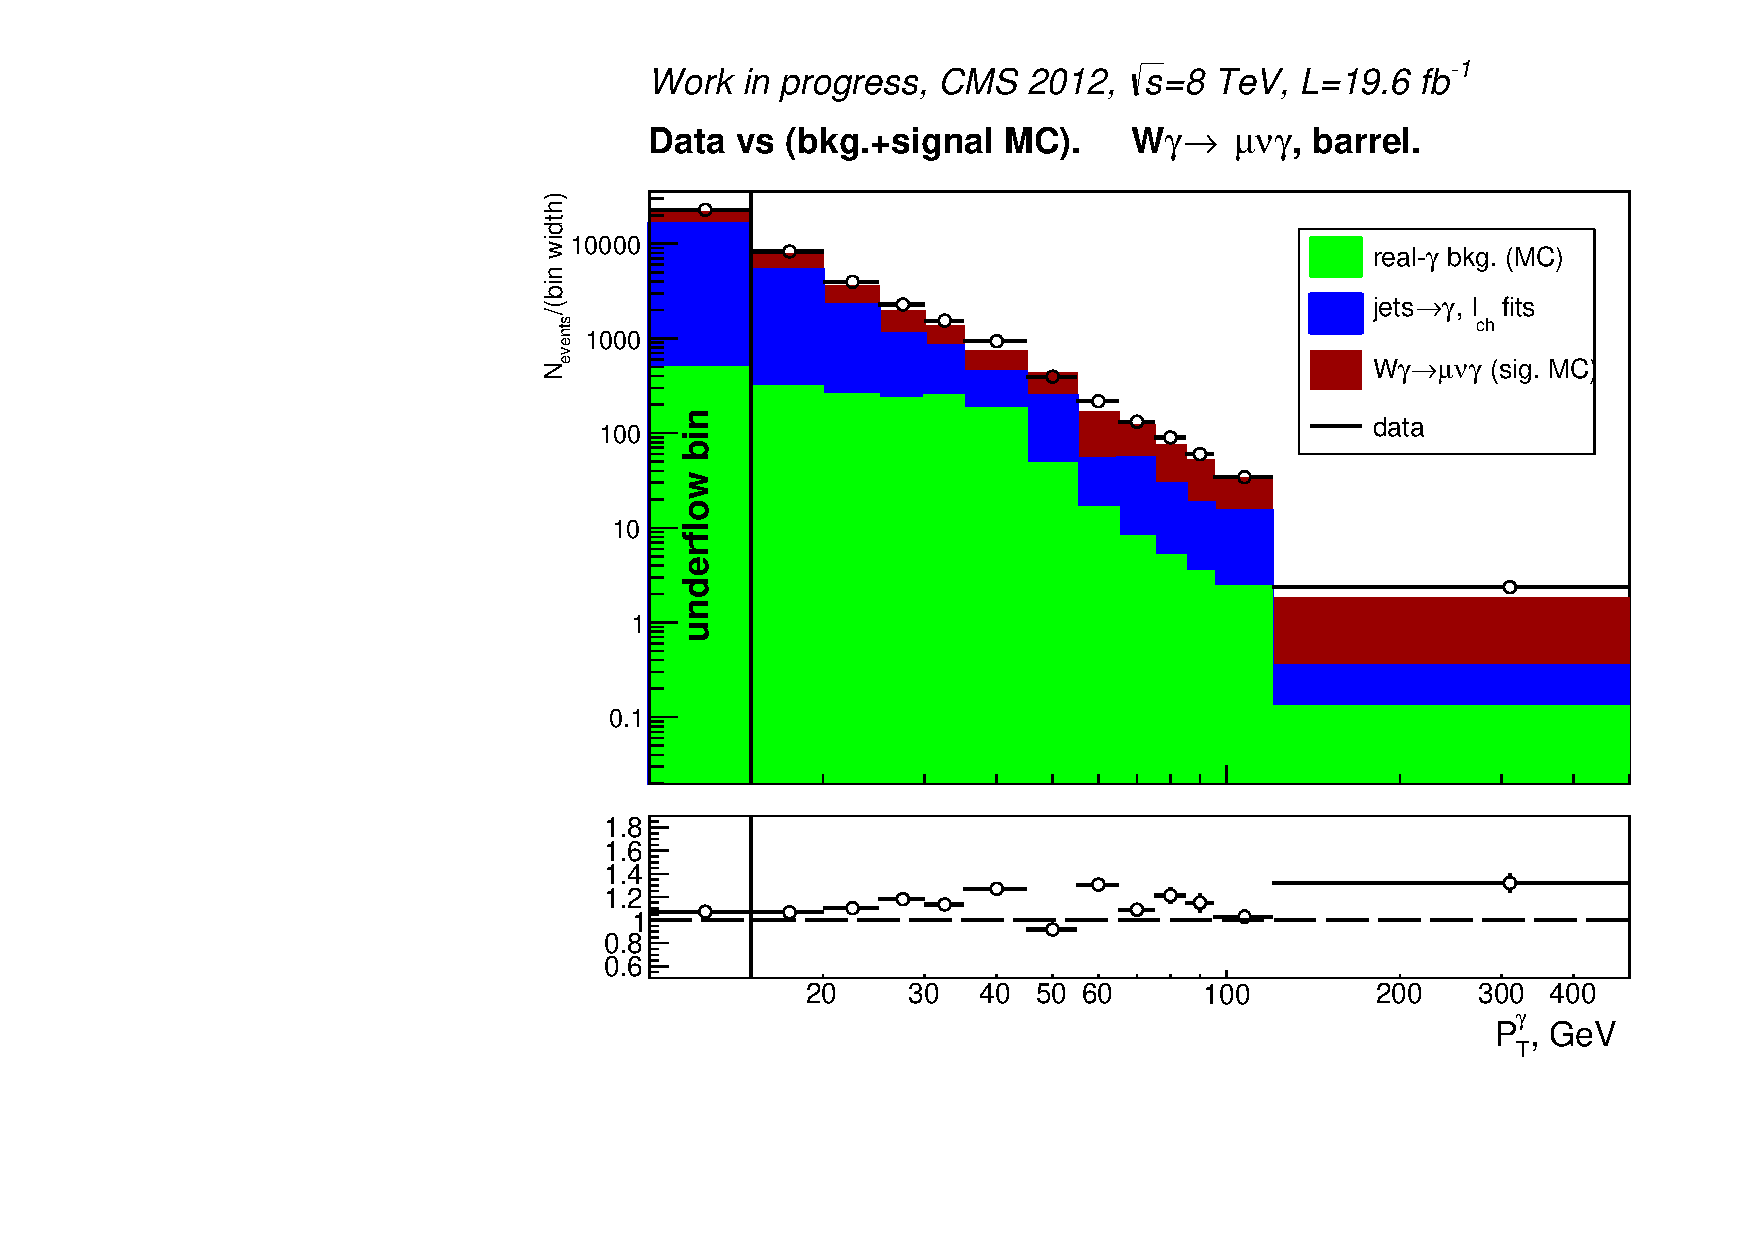
\includegraphics[width=0.45\textwidth]{../figs/figs_v11/MUON_WGamma/PrepareYields/c_DATAvsBkgPlusSigMCc_MUON_WGamma_TEMPL_CHISO_UNblind__Barrel__phoEt.pdf}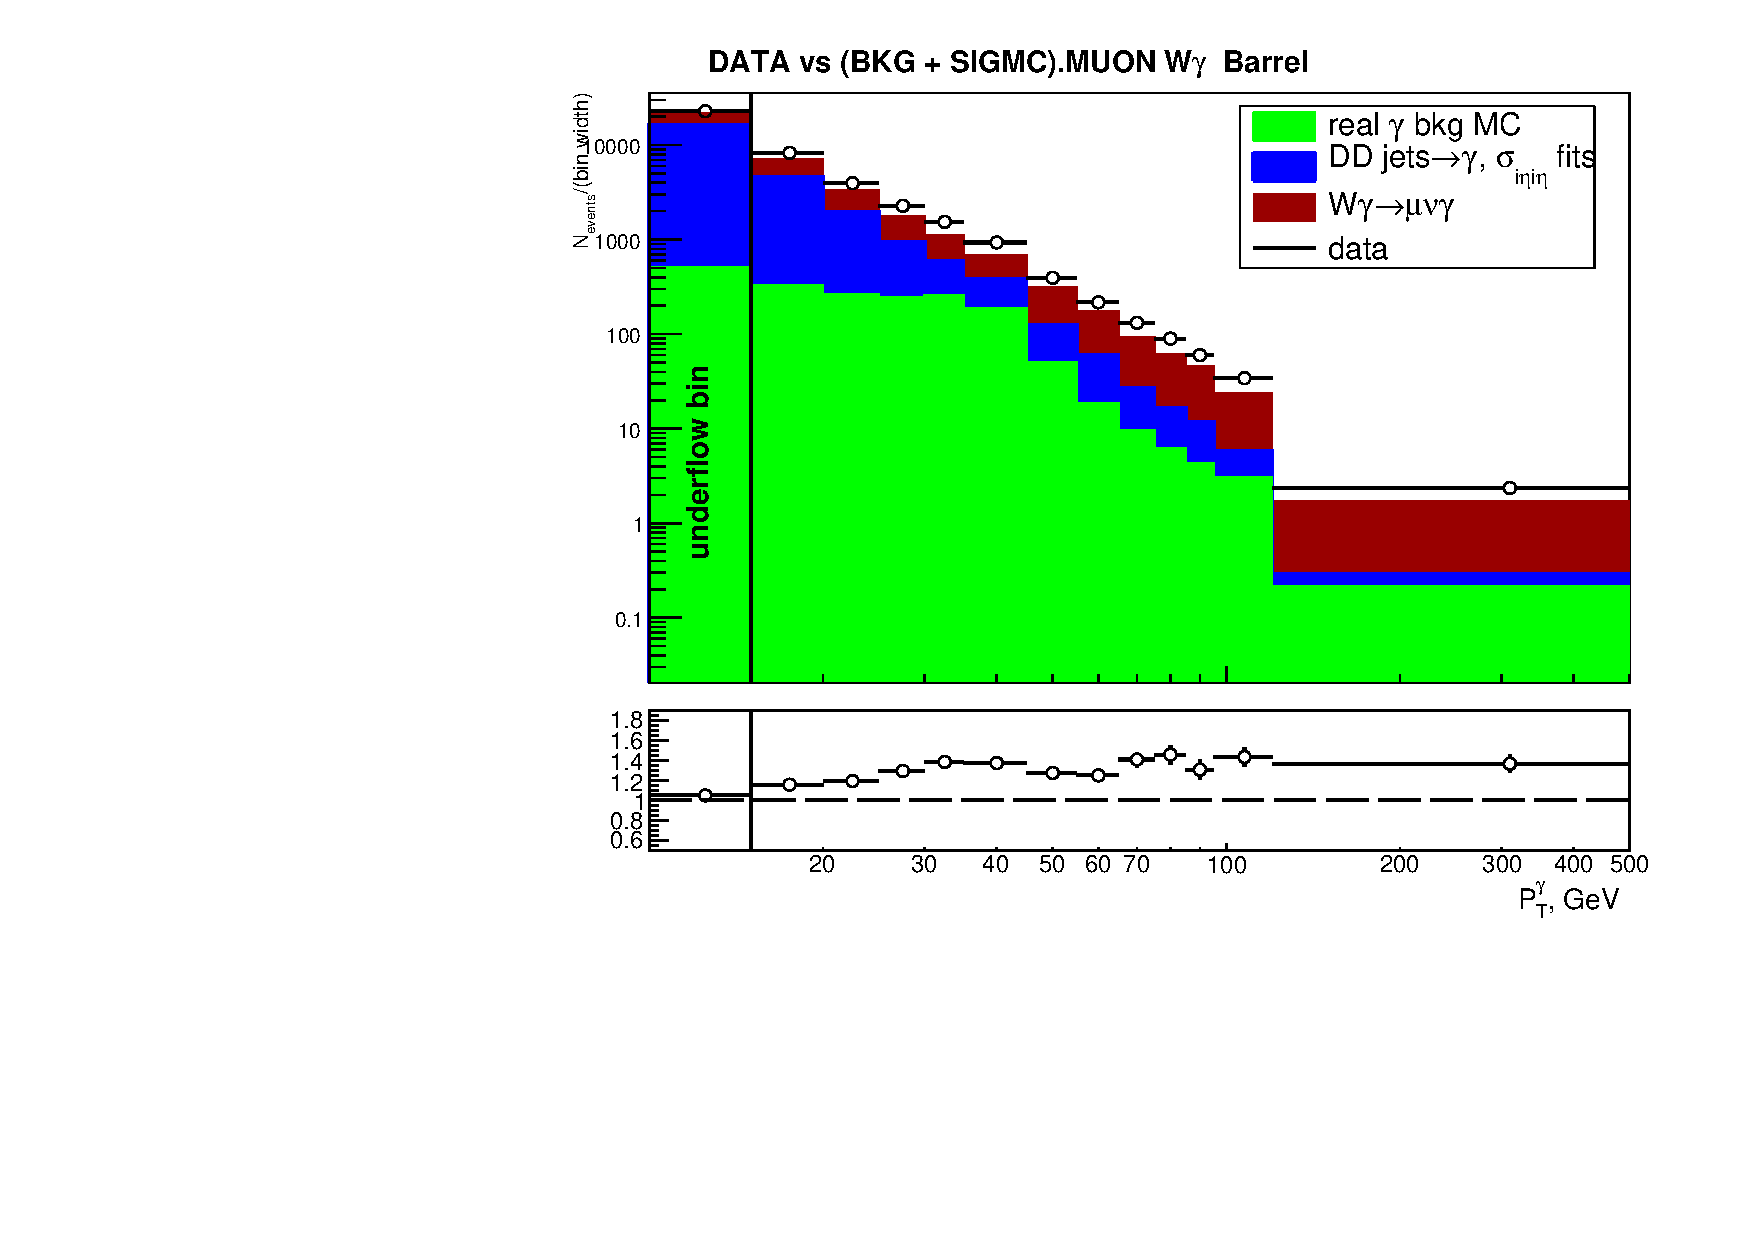
\includegraphics[width=0.45\textwidth]{../figs/figs_v11/MUON_WGamma/PrepareYields/c_DATAvsBkgPlusSigMCc_MUON_WGamma_TEMPL_SIHIH_UNblind__Barrel__phoEt.pdf}\\
       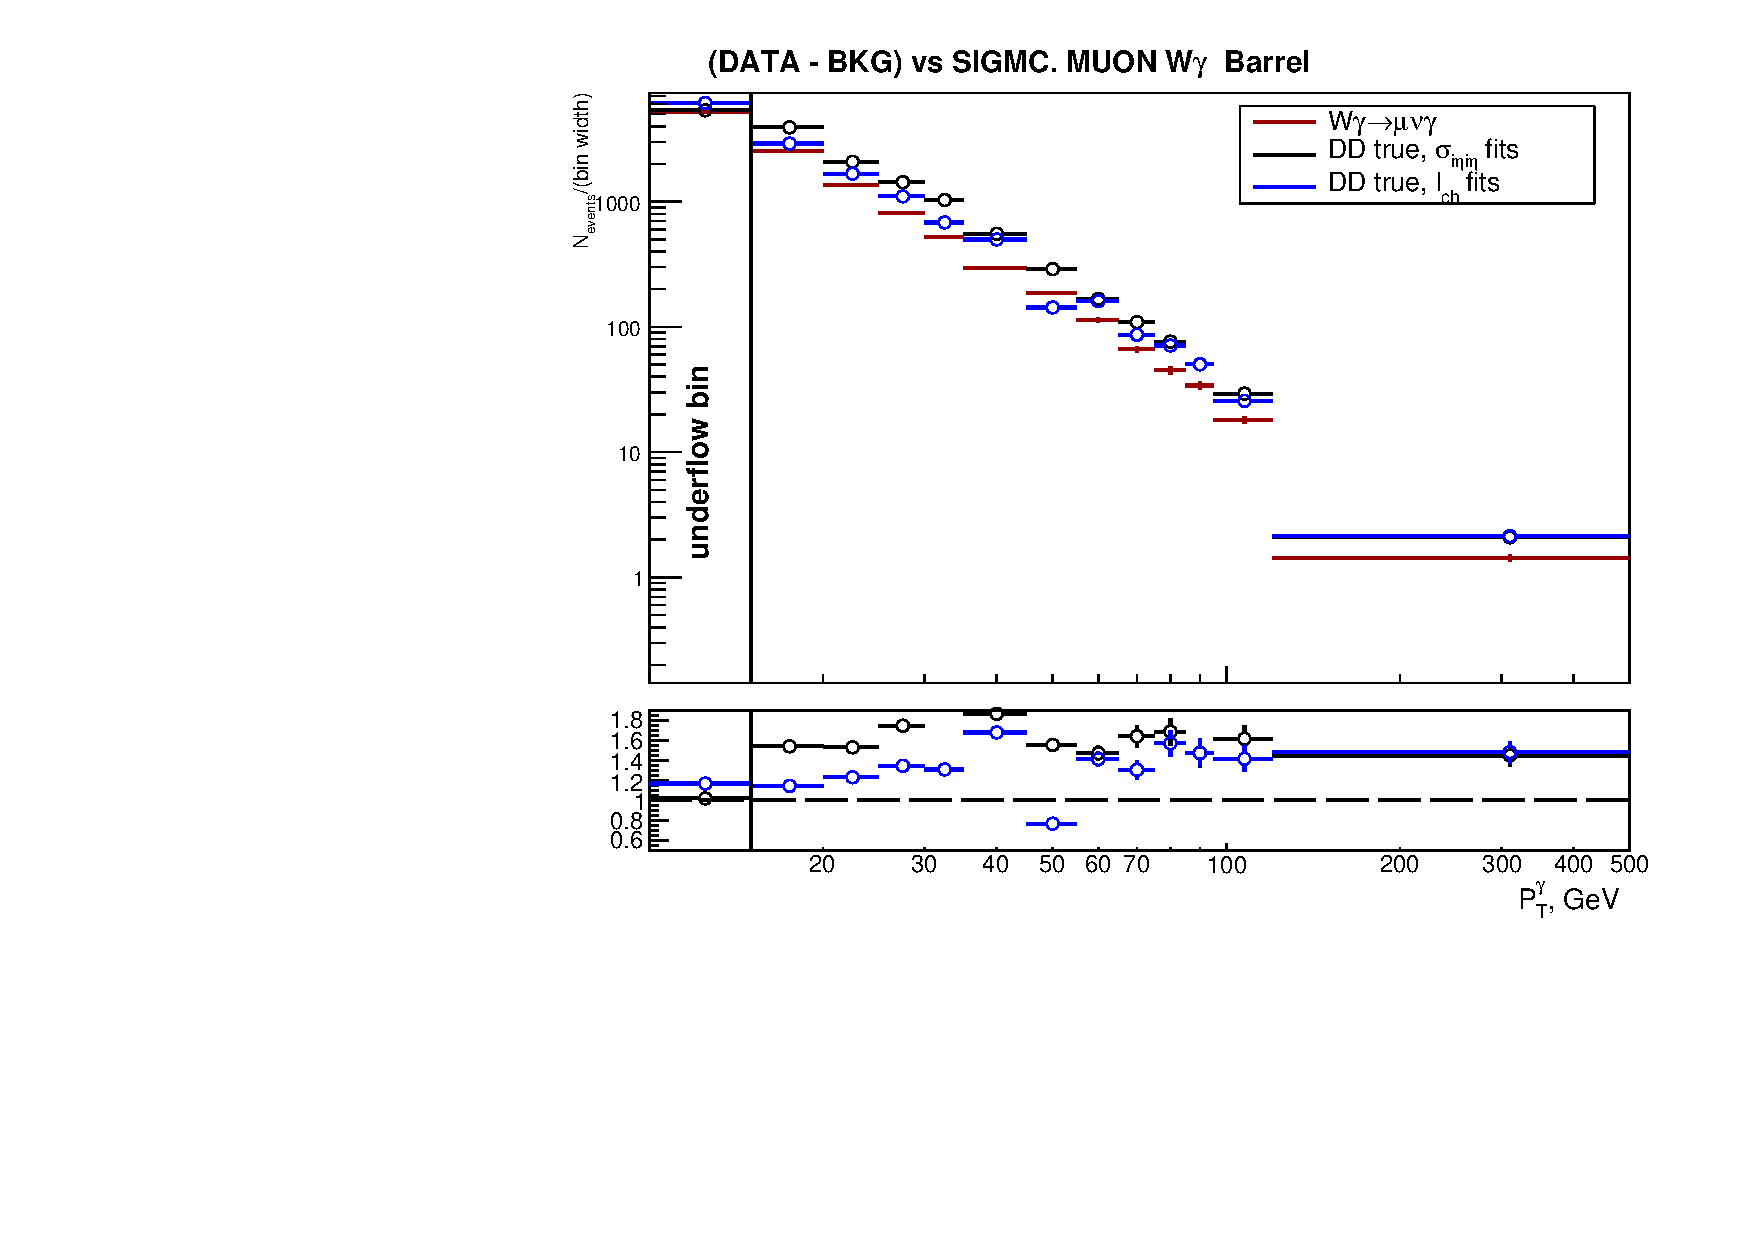
\includegraphics[width=0.45\textwidth]{../figs/figs_v11/MUON_WGamma/PrepareYields/c_BkgSubtrDATAvsSIGMC_c_MUON_WGamma__UNblind__Barrel__phoEt.pdf}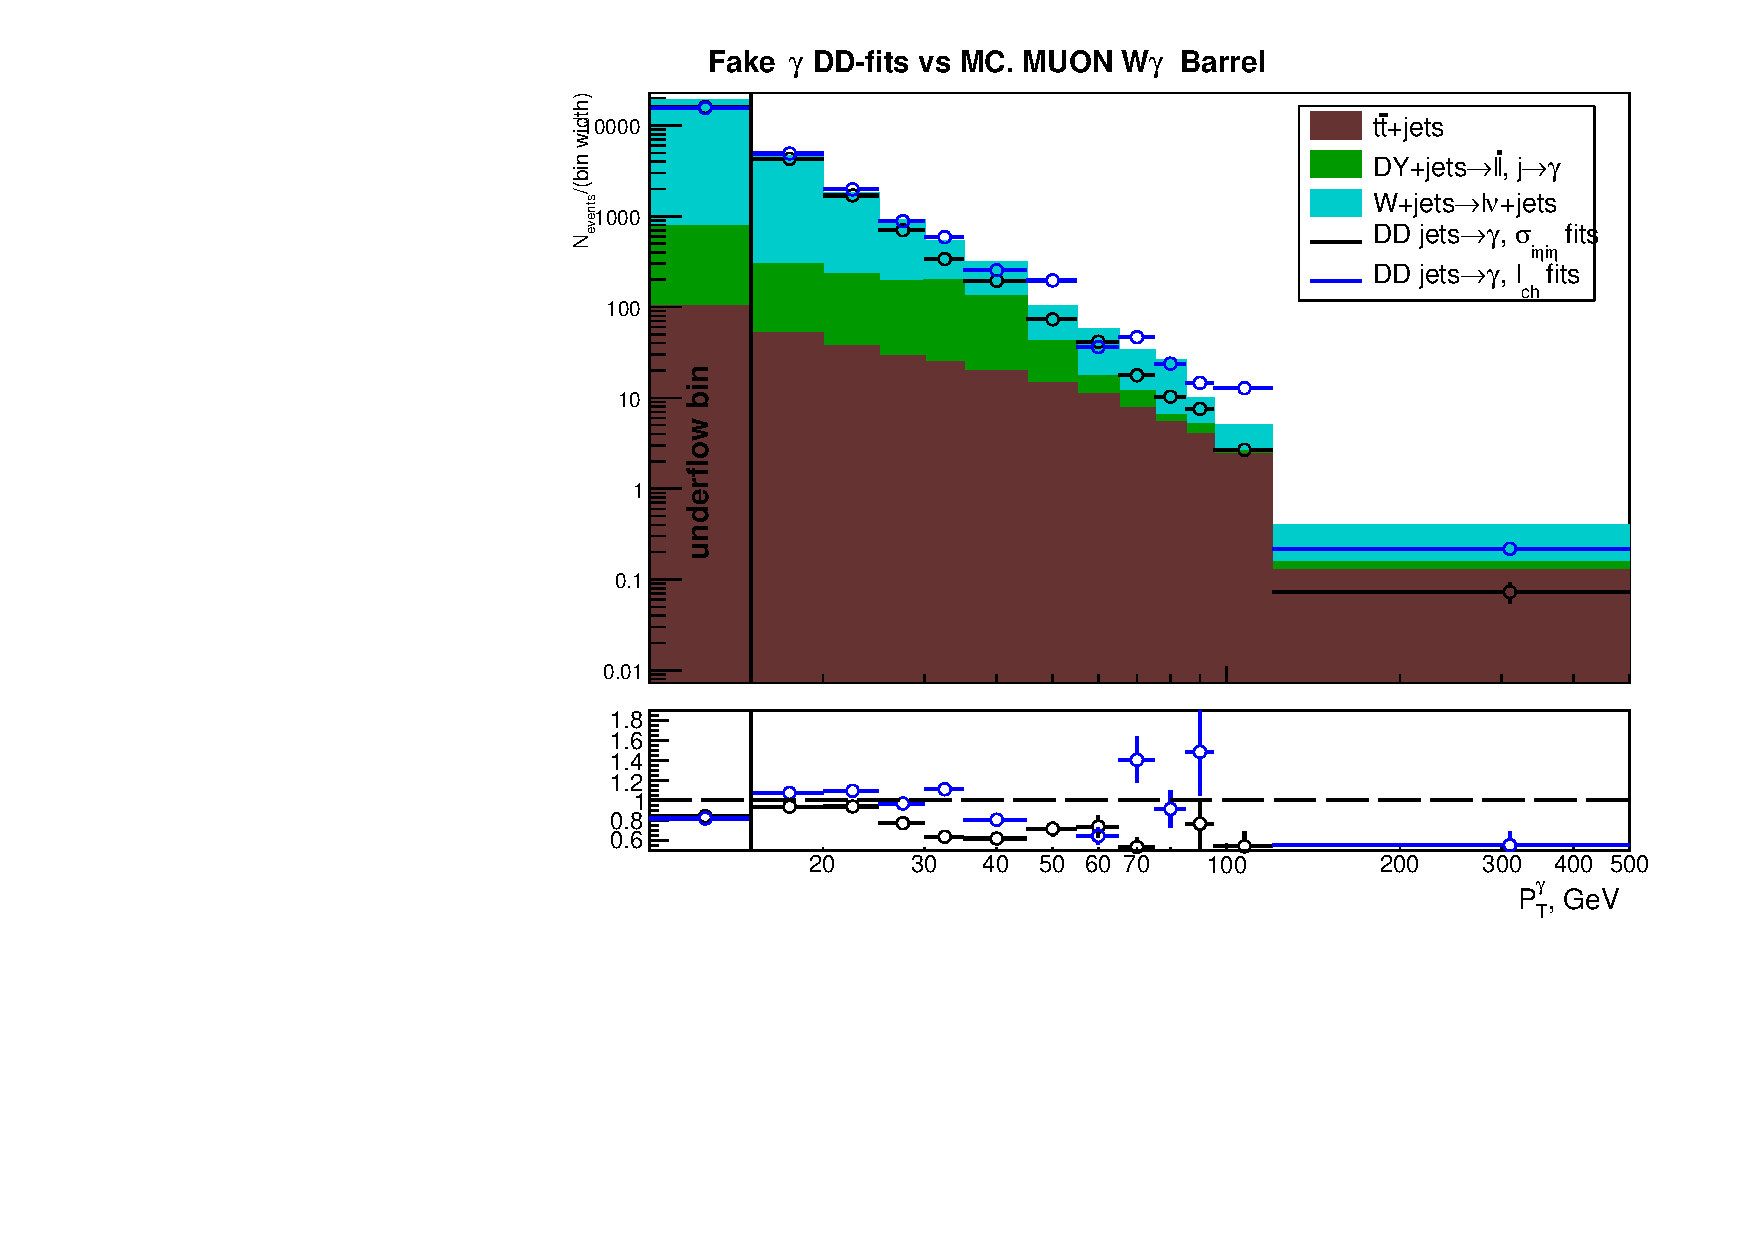
\includegraphics[width=0.45\textwidth]{../figs/figs_v11/MUON_WGamma/PrepareYields/c_FakeDDvsMC_c_MUON_WGamma__UNblind__Barrel__phoEt.pdf}\\
    \end{center}
  \end{figure}
\end{frame}%{$jets \rightarrow \gamma$ Background Subtraction. Plots, W$\gamma$}

\begin{frame}\frametitle{\footnotesize{$P_T^{\gamma}$ Spectrum before and after Background Subtraction. Muon Channel, Endcap}}
  \tiny{Top: data vs fake-$\gamma$ background derived from the template method + real-$\gamma$ background predicted by dedicated MC samples + signal MC, with $I_{ch}$ and $\sigma_{i\eta{i}\eta}$ used as fit variables. Bottom: left: data yields after full background subtraction vs signal MC. $I_{ch}$ vs $\sigma_{i\eta{i}\eta}$ fit results. Right: fake-$\gamma$ data driven background prediction vs MC. Plotted with the stat error only.}
  \begin{figure}[htb]
    \begin{center}
    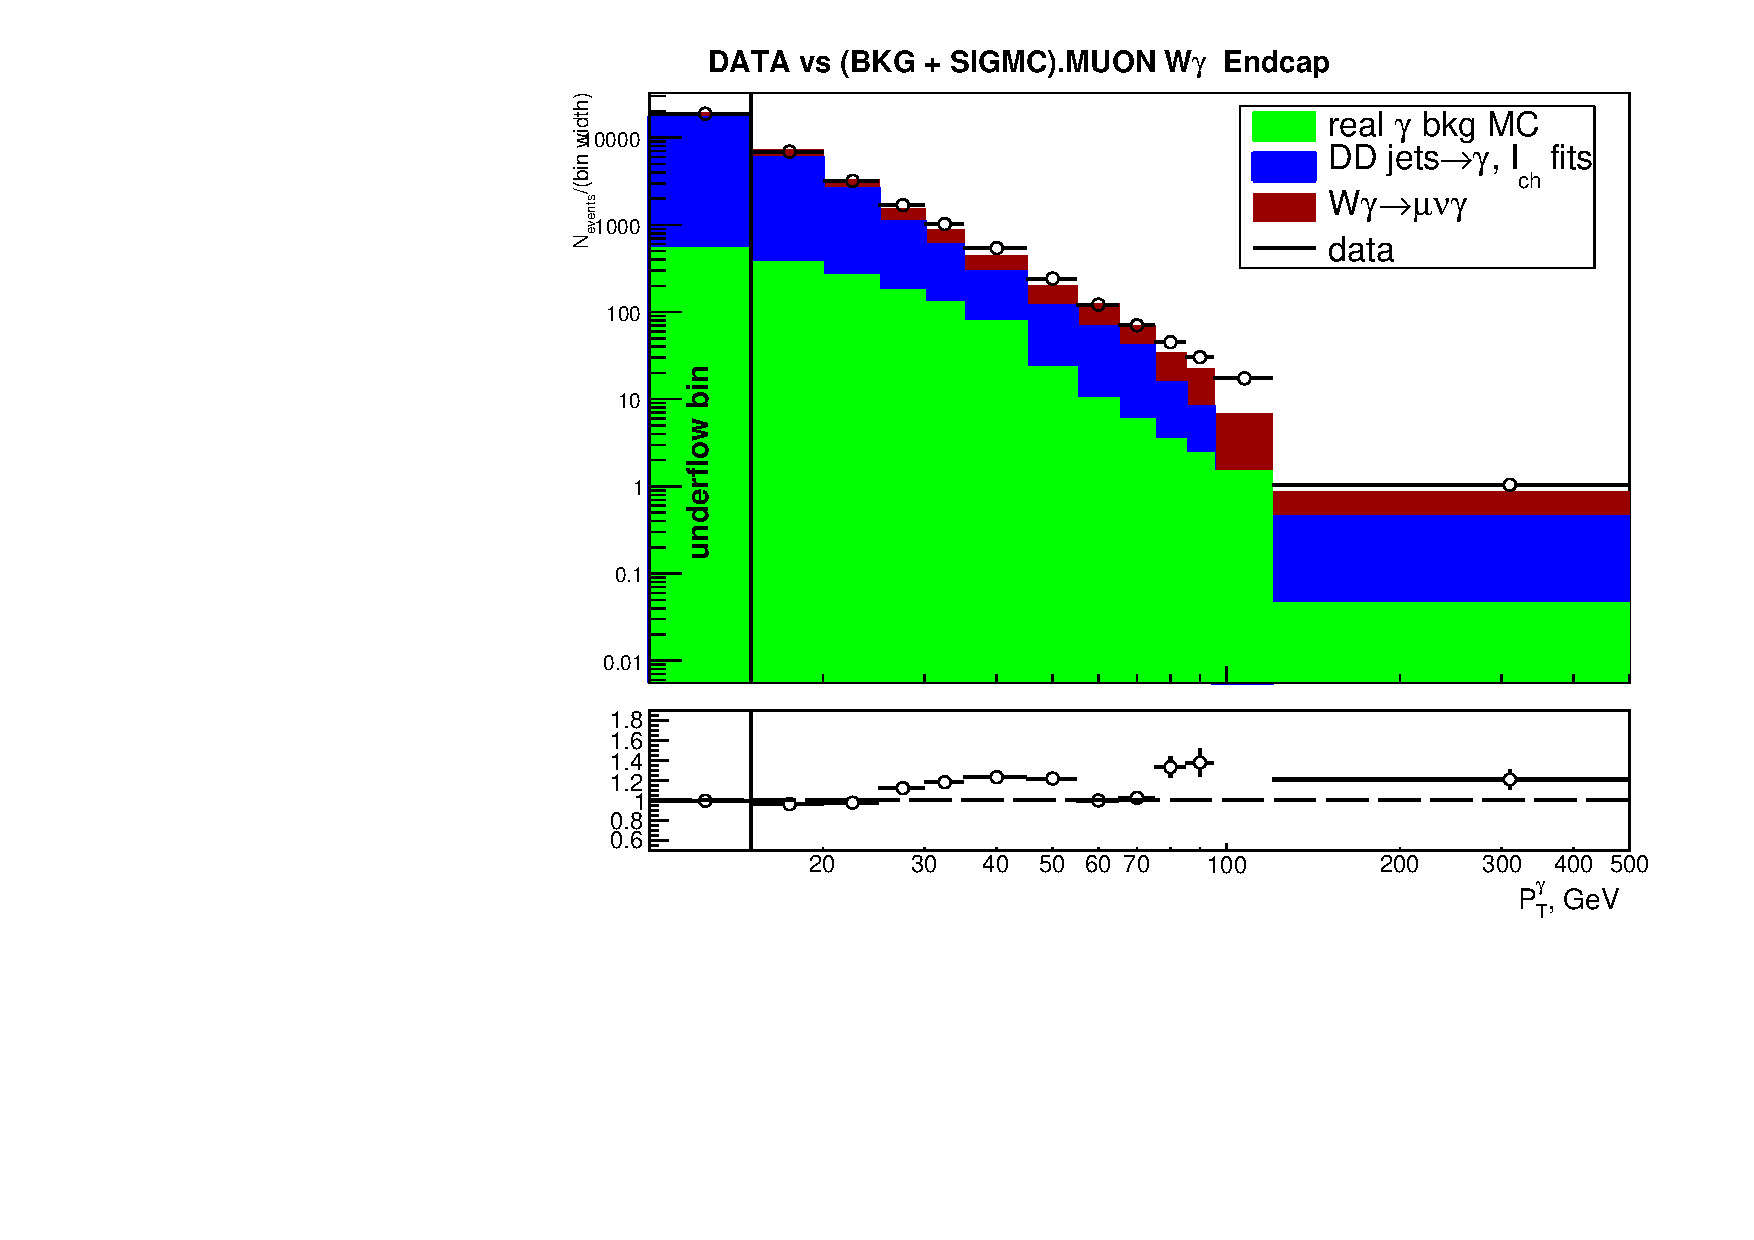
\includegraphics[width=0.45\textwidth]{../figs/figs_v11/MUON_WGamma/PrepareYields/c_DATAvsBkgPlusSigMCc_MUON_WGamma_TEMPL_CHISO_UNblind__Endcap__phoEt.pdf}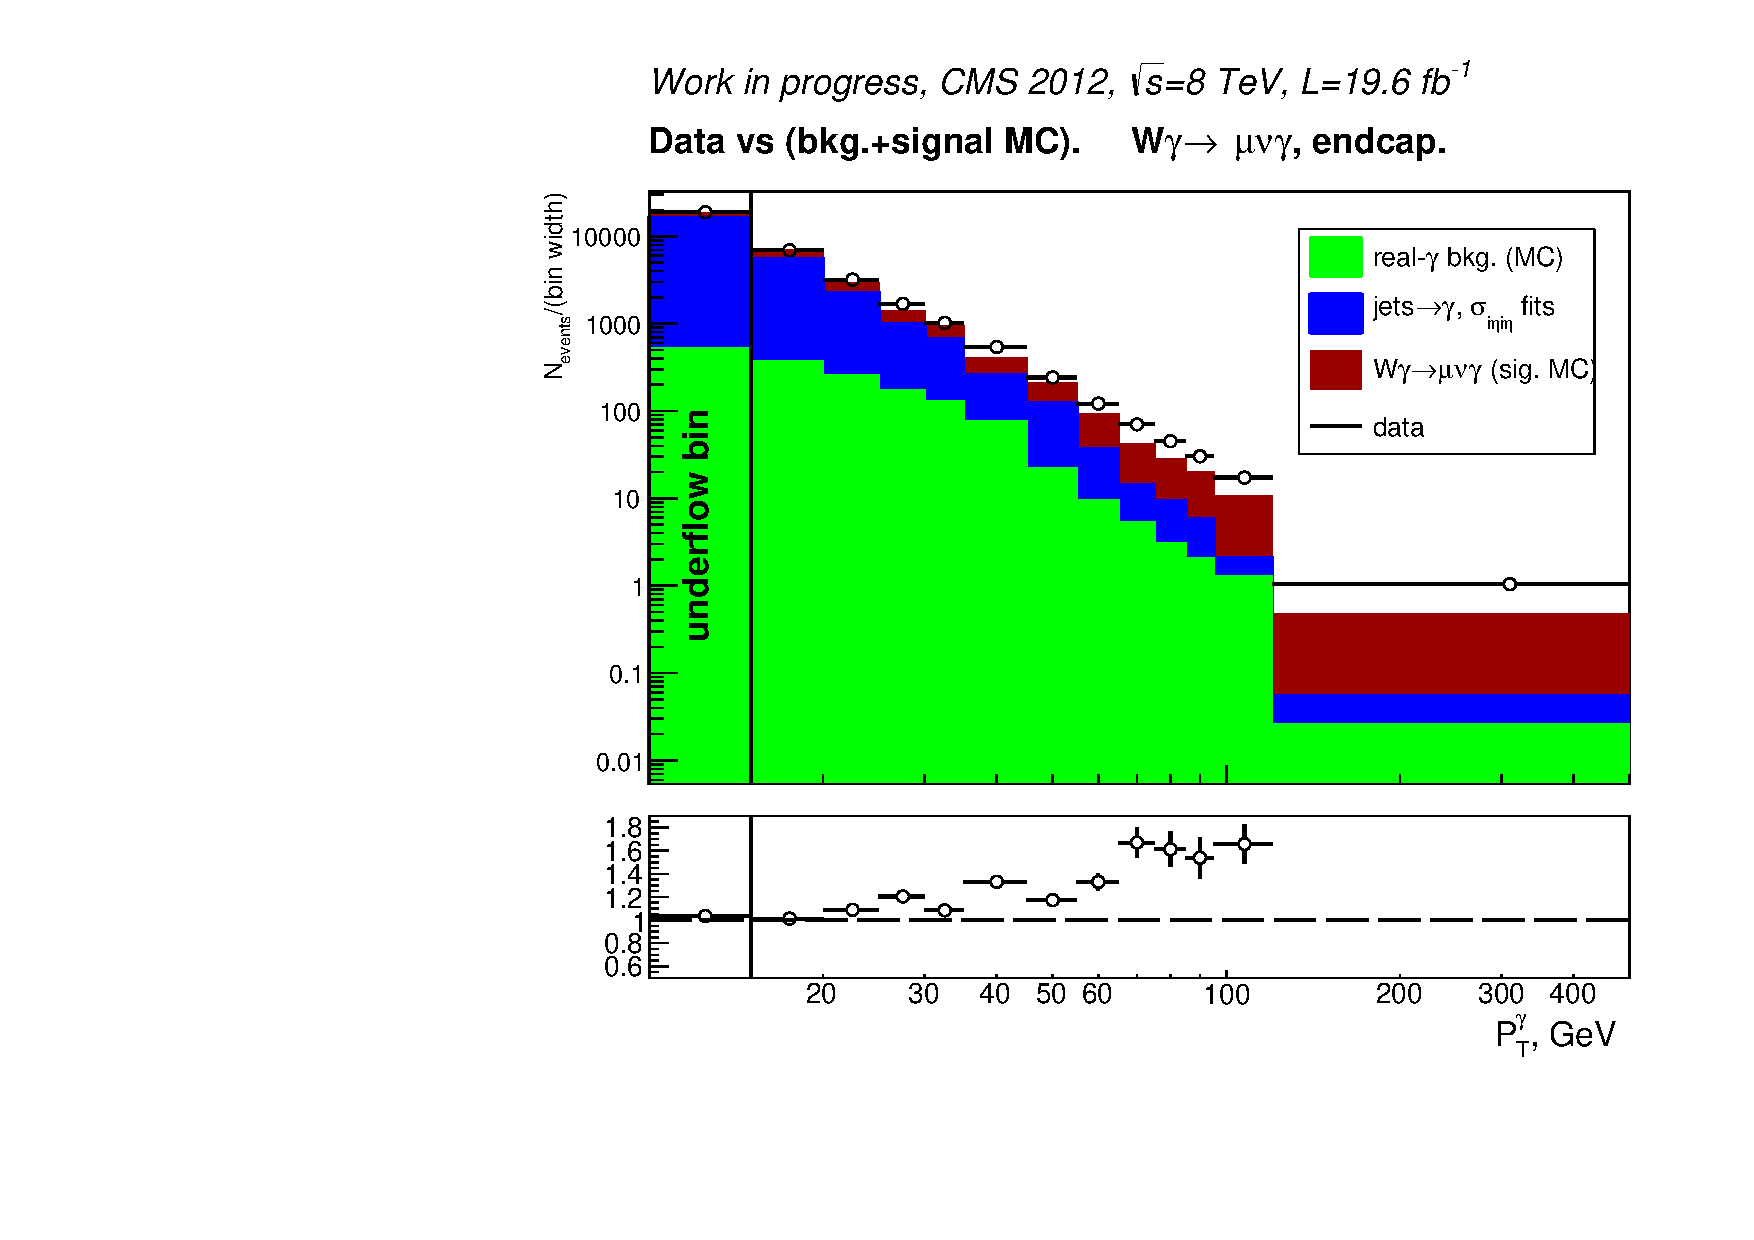
\includegraphics[width=0.45\textwidth]{../figs/figs_v11/MUON_WGamma/PrepareYields/c_DATAvsBkgPlusSigMCc_MUON_WGamma_TEMPL_SIHIH_UNblind__Endcap__phoEt.pdf}\\
    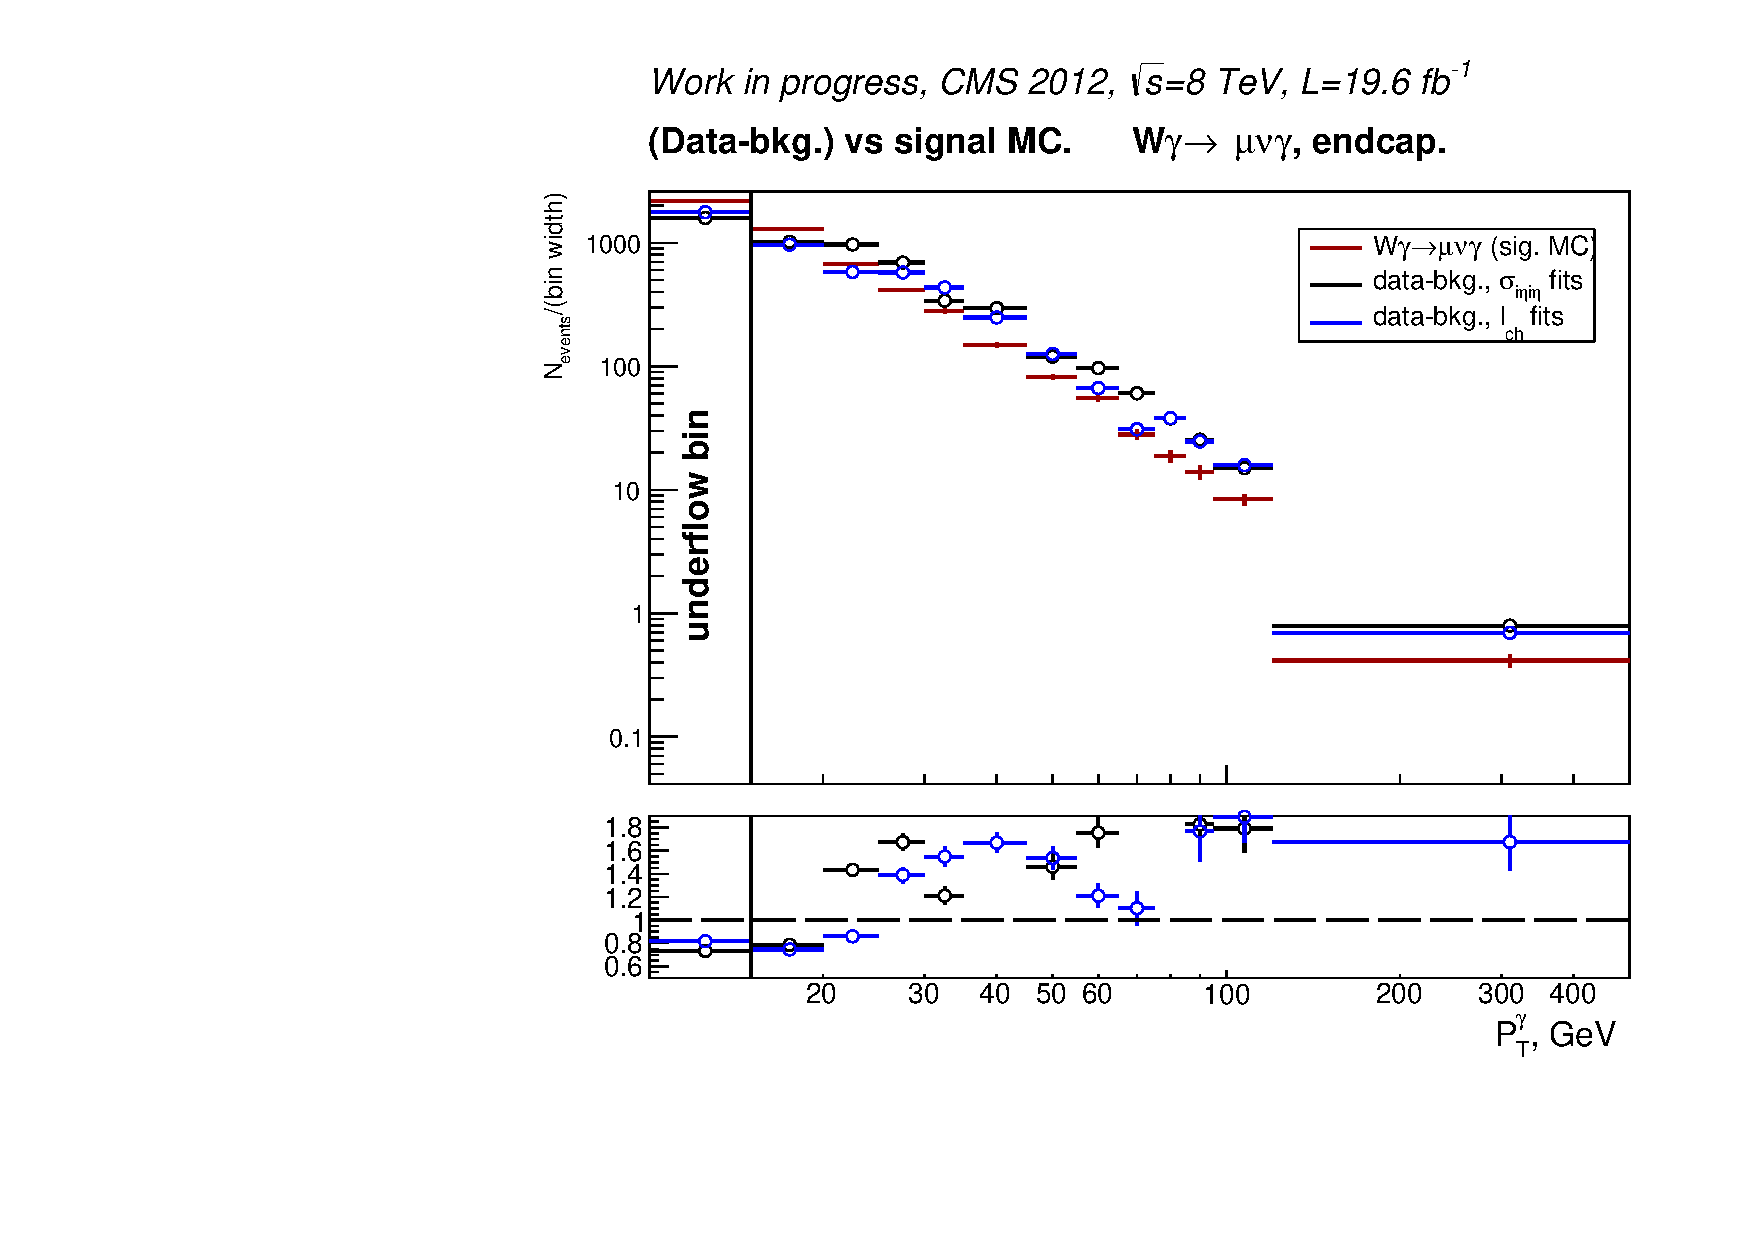
\includegraphics[width=0.45\textwidth]{../figs/figs_v11/MUON_WGamma/PrepareYields/c_BkgSubtrDATAvsSIGMC_c_MUON_WGamma__UNblind__Endcap__phoEt.pdf}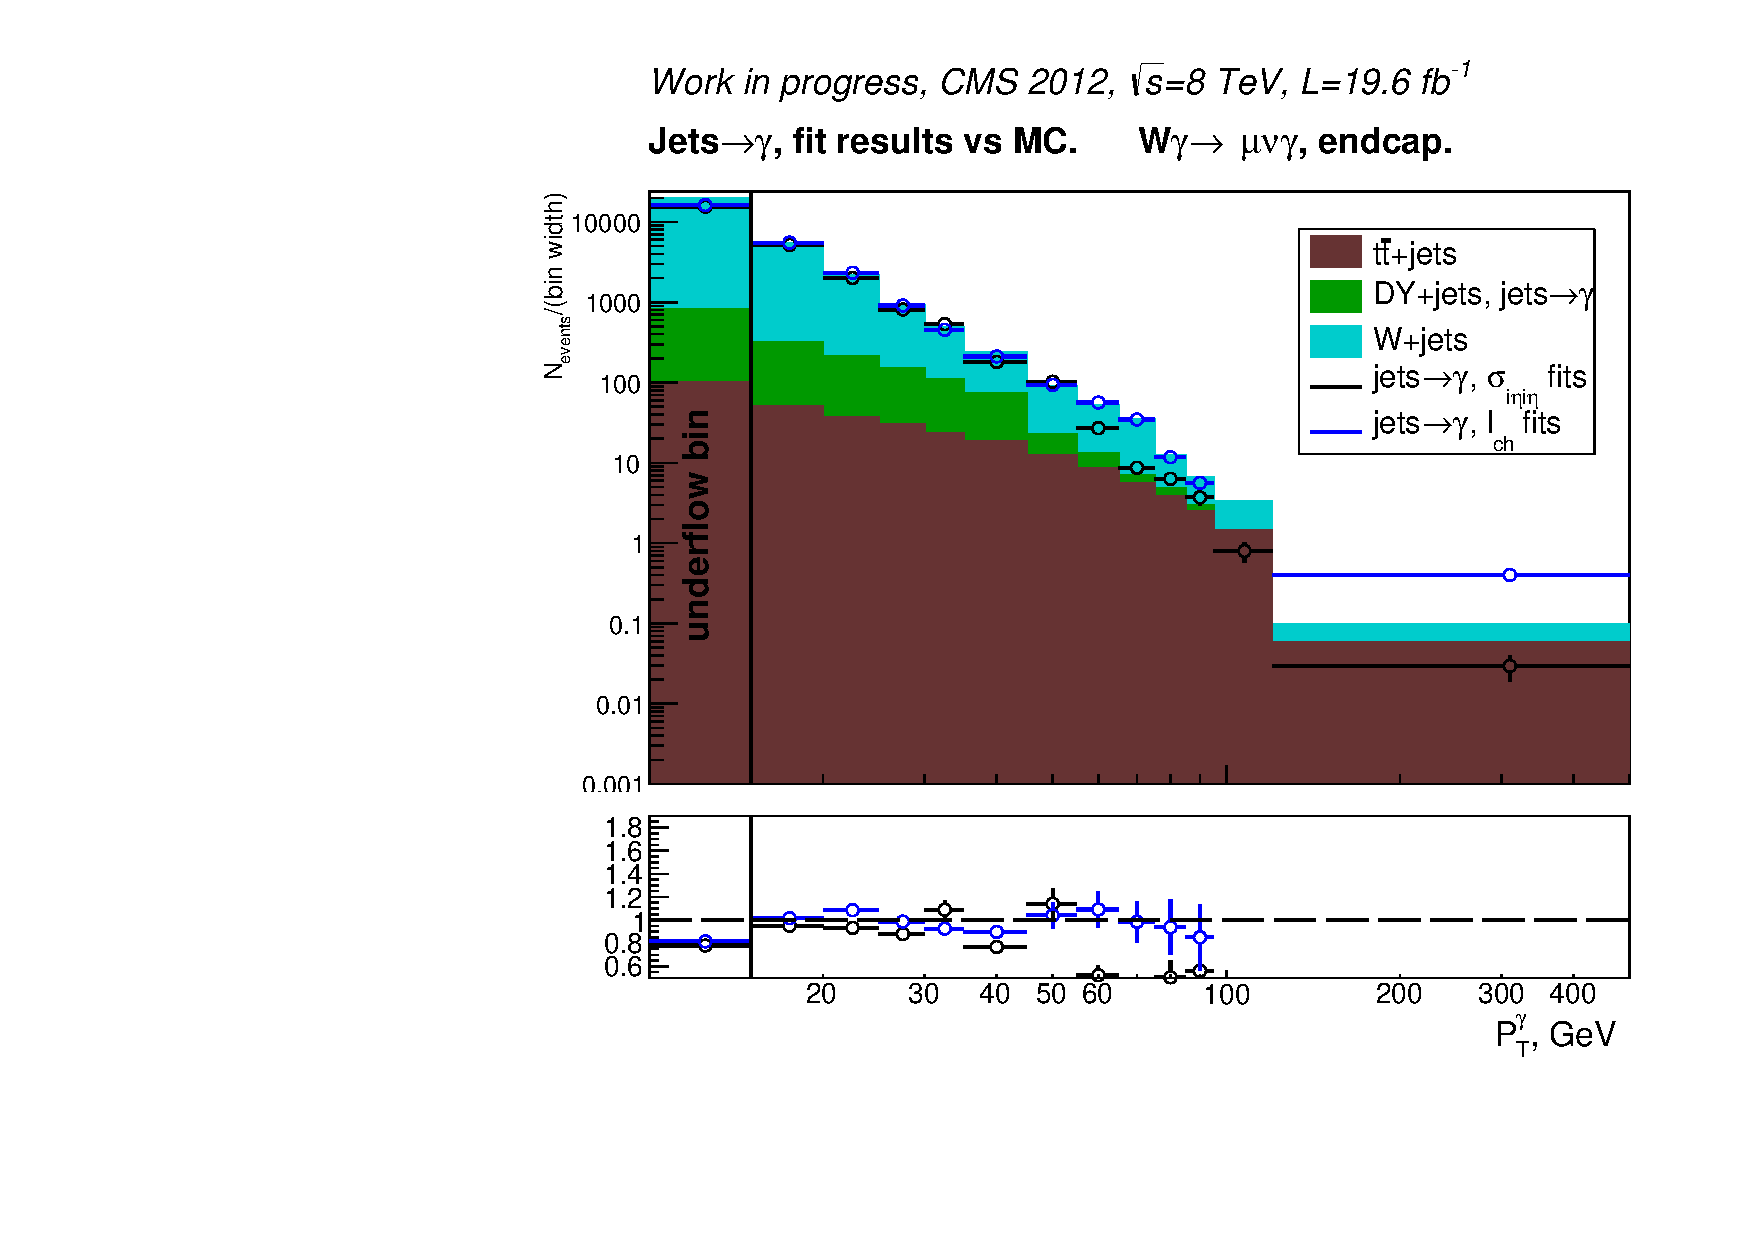
\includegraphics[width=0.45\textwidth]{../figs/figs_v11/MUON_WGamma/PrepareYields/c_FakeDDvsMC_c_MUON_WGamma__UNblind__Endcap__phoEt.pdf}\\
    \end{center}
  \end{figure}
\end{frame}%{$jets \rightarrow \gamma$ Background Subtraction. Plots, W$\gamma$}

\begin{frame}\frametitle{\footnotesize{$P_T^{\gamma}$ Spectrum before and after Background Subtraction. Electron Channel, Barrel}}
  \tiny{Top: data vs fake-$\gamma$ background derived from the template method + real-$\gamma$ background predicted by dedicated MC samples + signal MC, with $I_{ch}$ and $\sigma_{i\eta{i}\eta}$ used as fit variables. Bottom: left: data yields after full background subtraction vs signal MC. $I_{ch}$ vs $\sigma_{i\eta{i}\eta}$ fit results. Right: fake-$\gamma$ data driven background prediction vs MC. Plotted with the stat error only.}
  \begin{figure}[htb]
    \begin{center}
       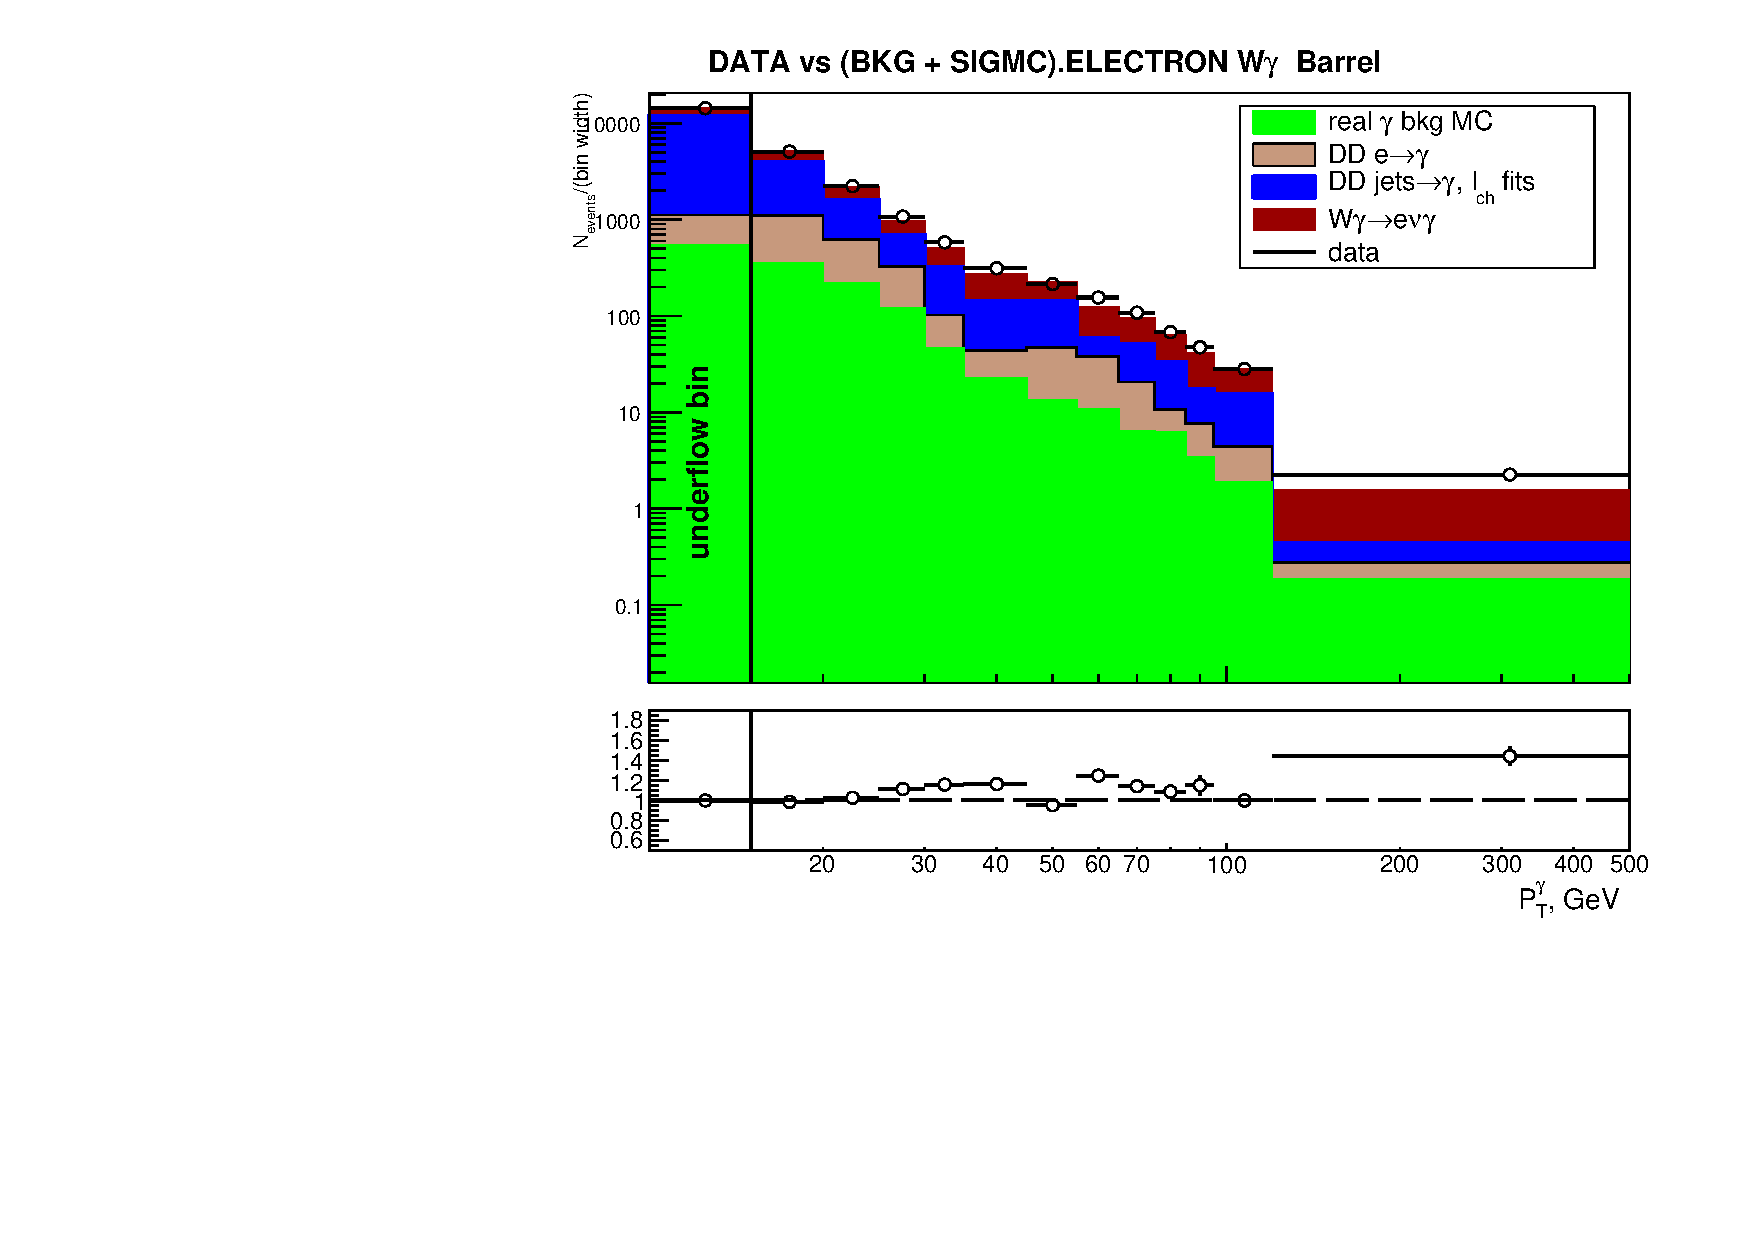
\includegraphics[width=0.45\textwidth]{../figs/figs_v11/ELECTRON_WGamma/PrepareYields/c_DATAvsBkgPlusSigMCc_ELECTRON_WGamma_TEMPL_CHISO_UNblind__Barrel__phoEt.pdf}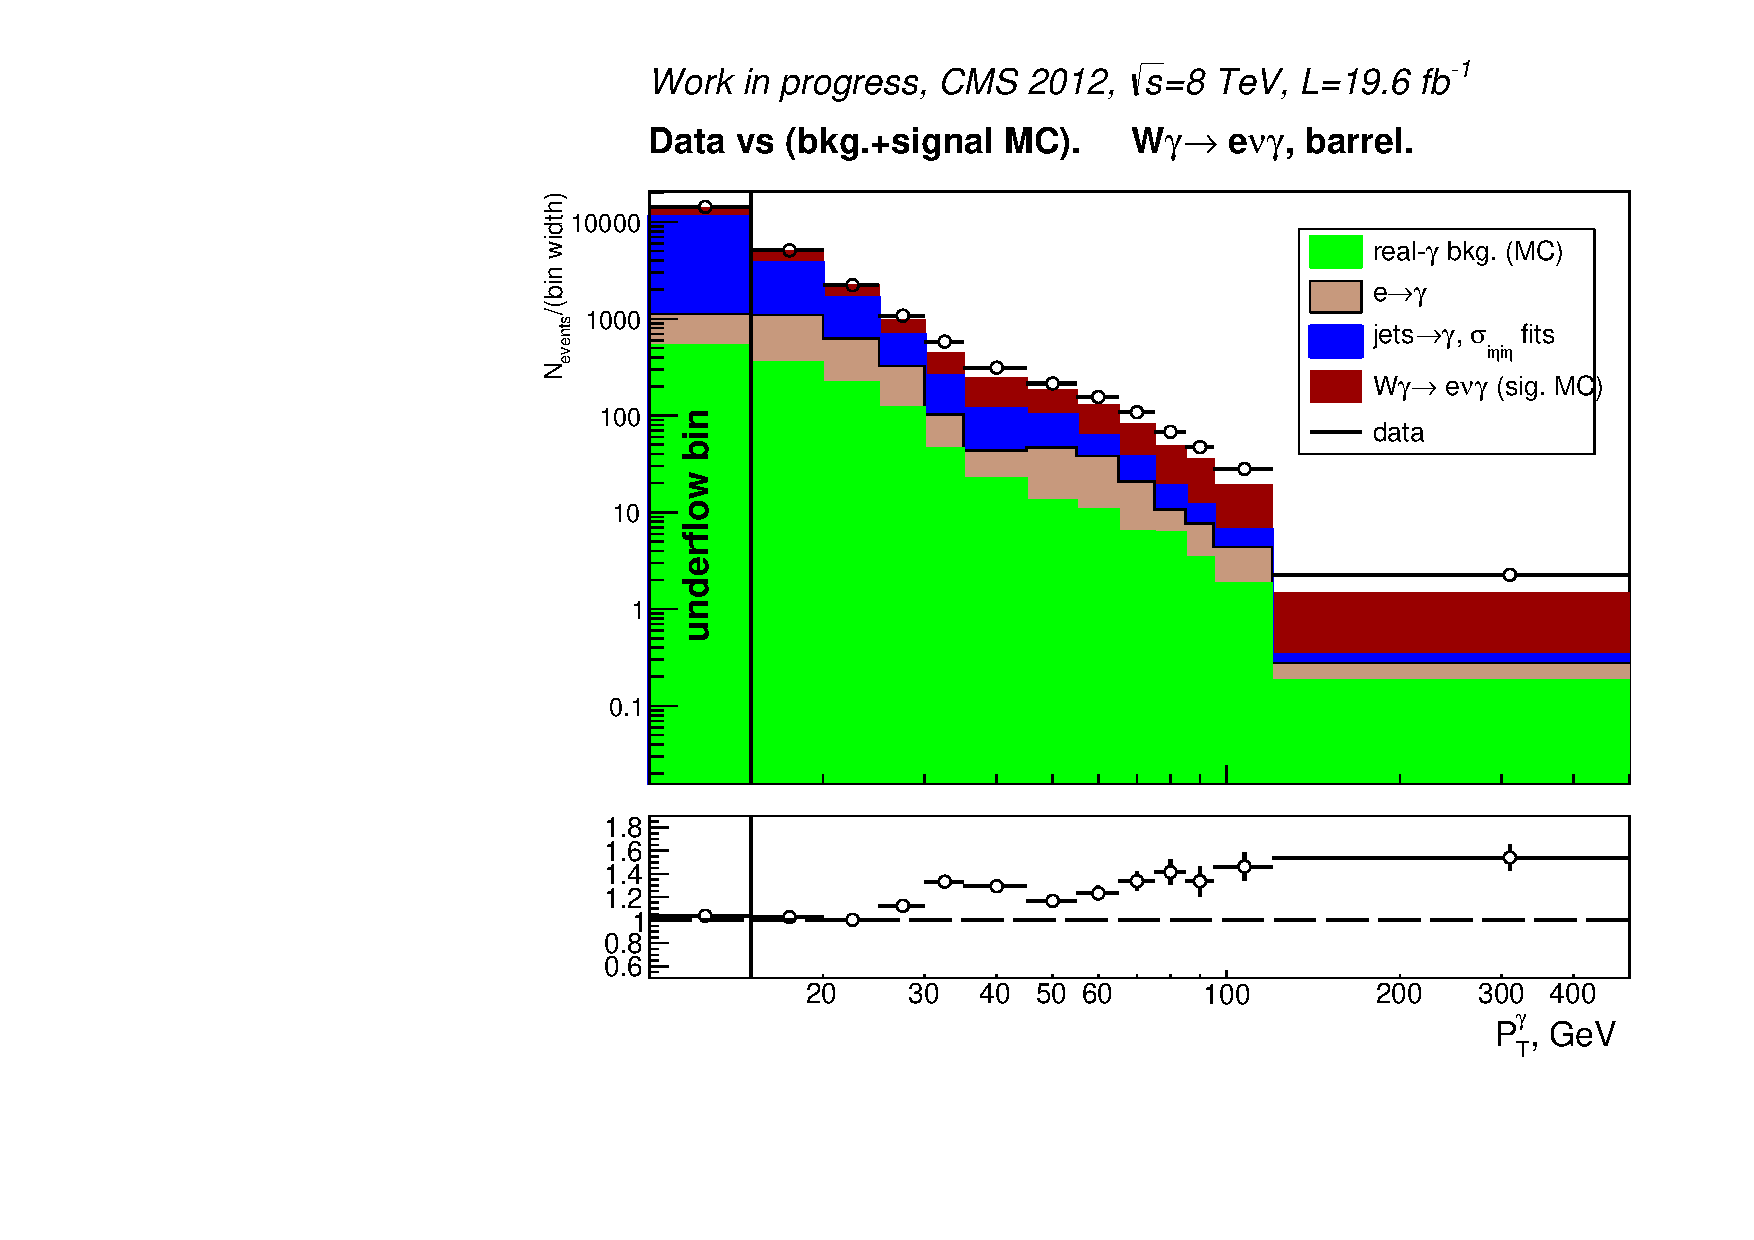
\includegraphics[width=0.45\textwidth]{../figs/figs_v11/ELECTRON_WGamma/PrepareYields/c_DATAvsBkgPlusSigMCc_ELECTRON_WGamma_TEMPL_SIHIH_UNblind__Barrel__phoEt.pdf}\\
       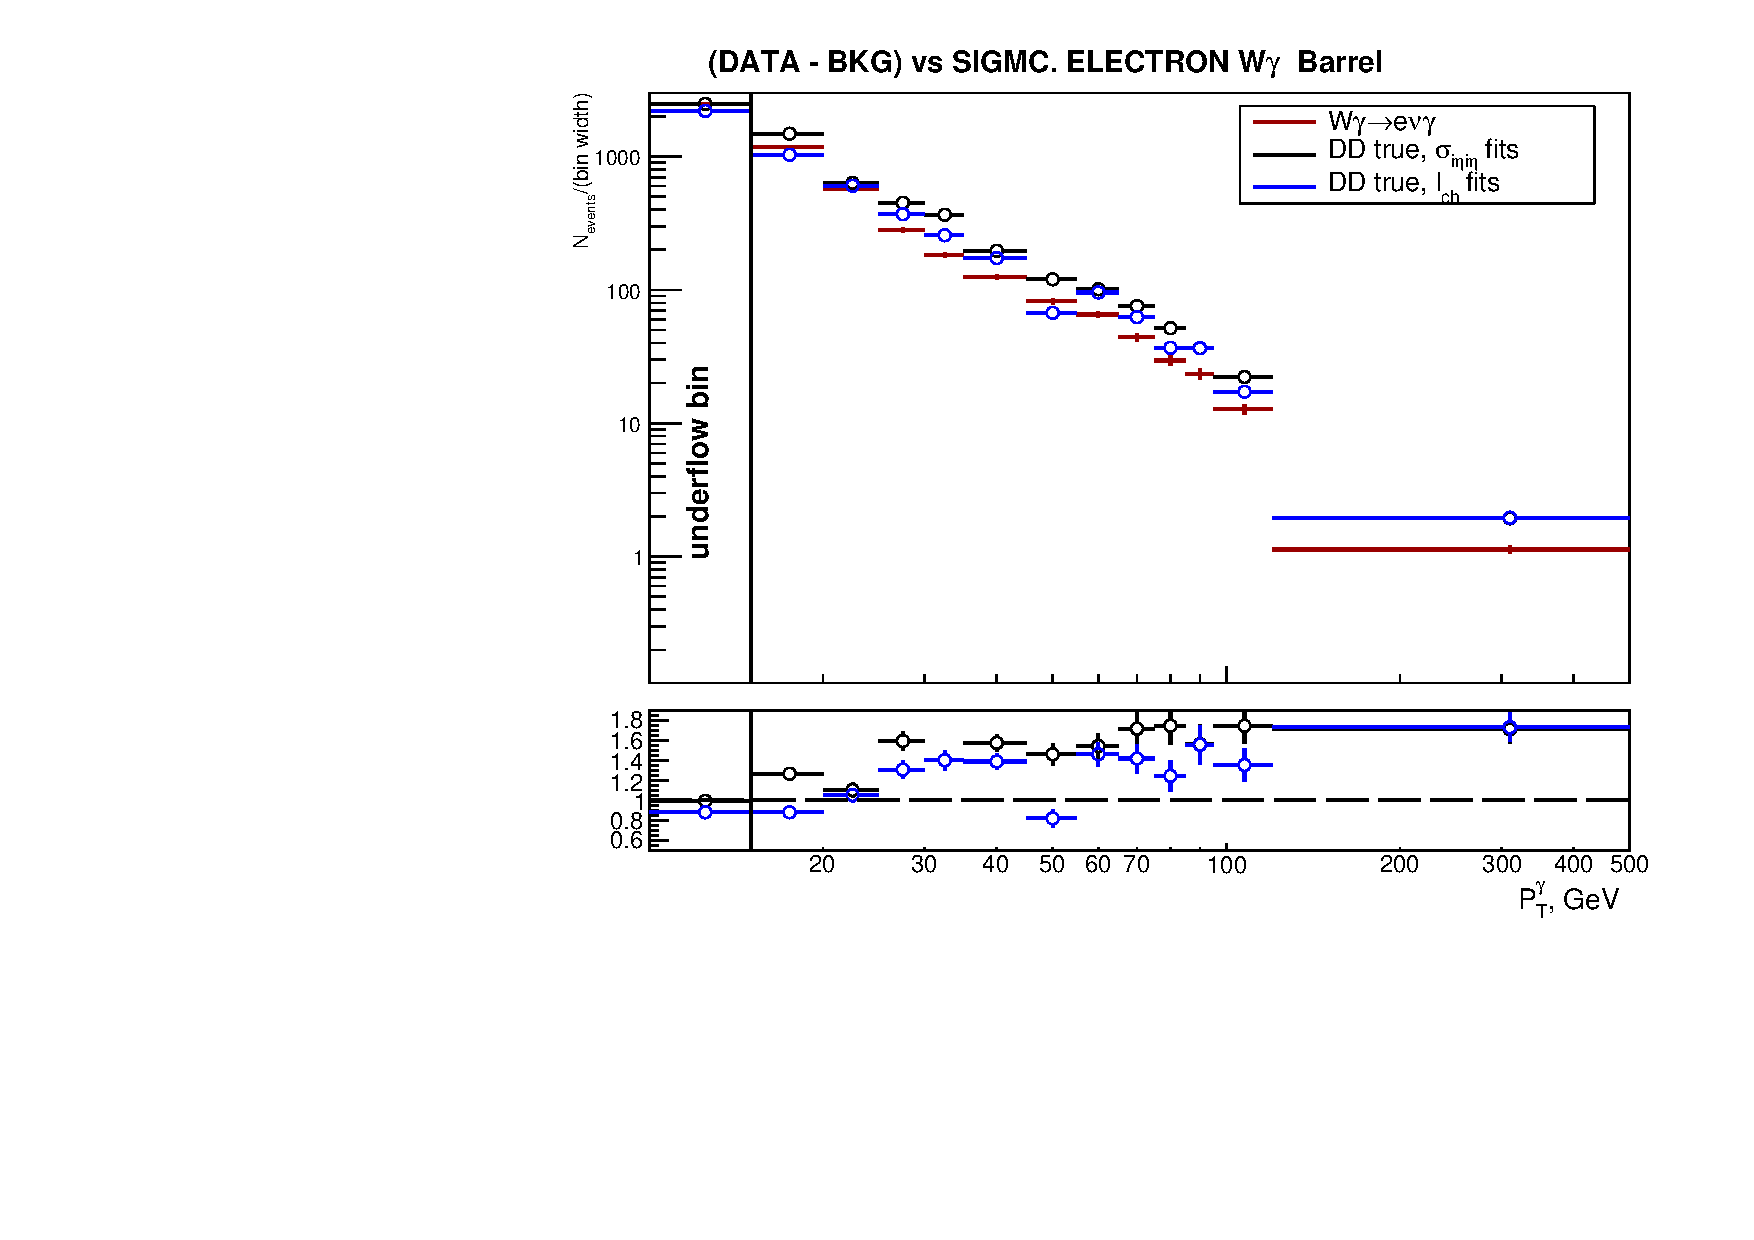
\includegraphics[width=0.45\textwidth]{../figs/figs_v11/ELECTRON_WGamma/PrepareYields/c_BkgSubtrDATAvsSIGMC_c_ELECTRON_WGamma__UNblind__Barrel__phoEt.pdf}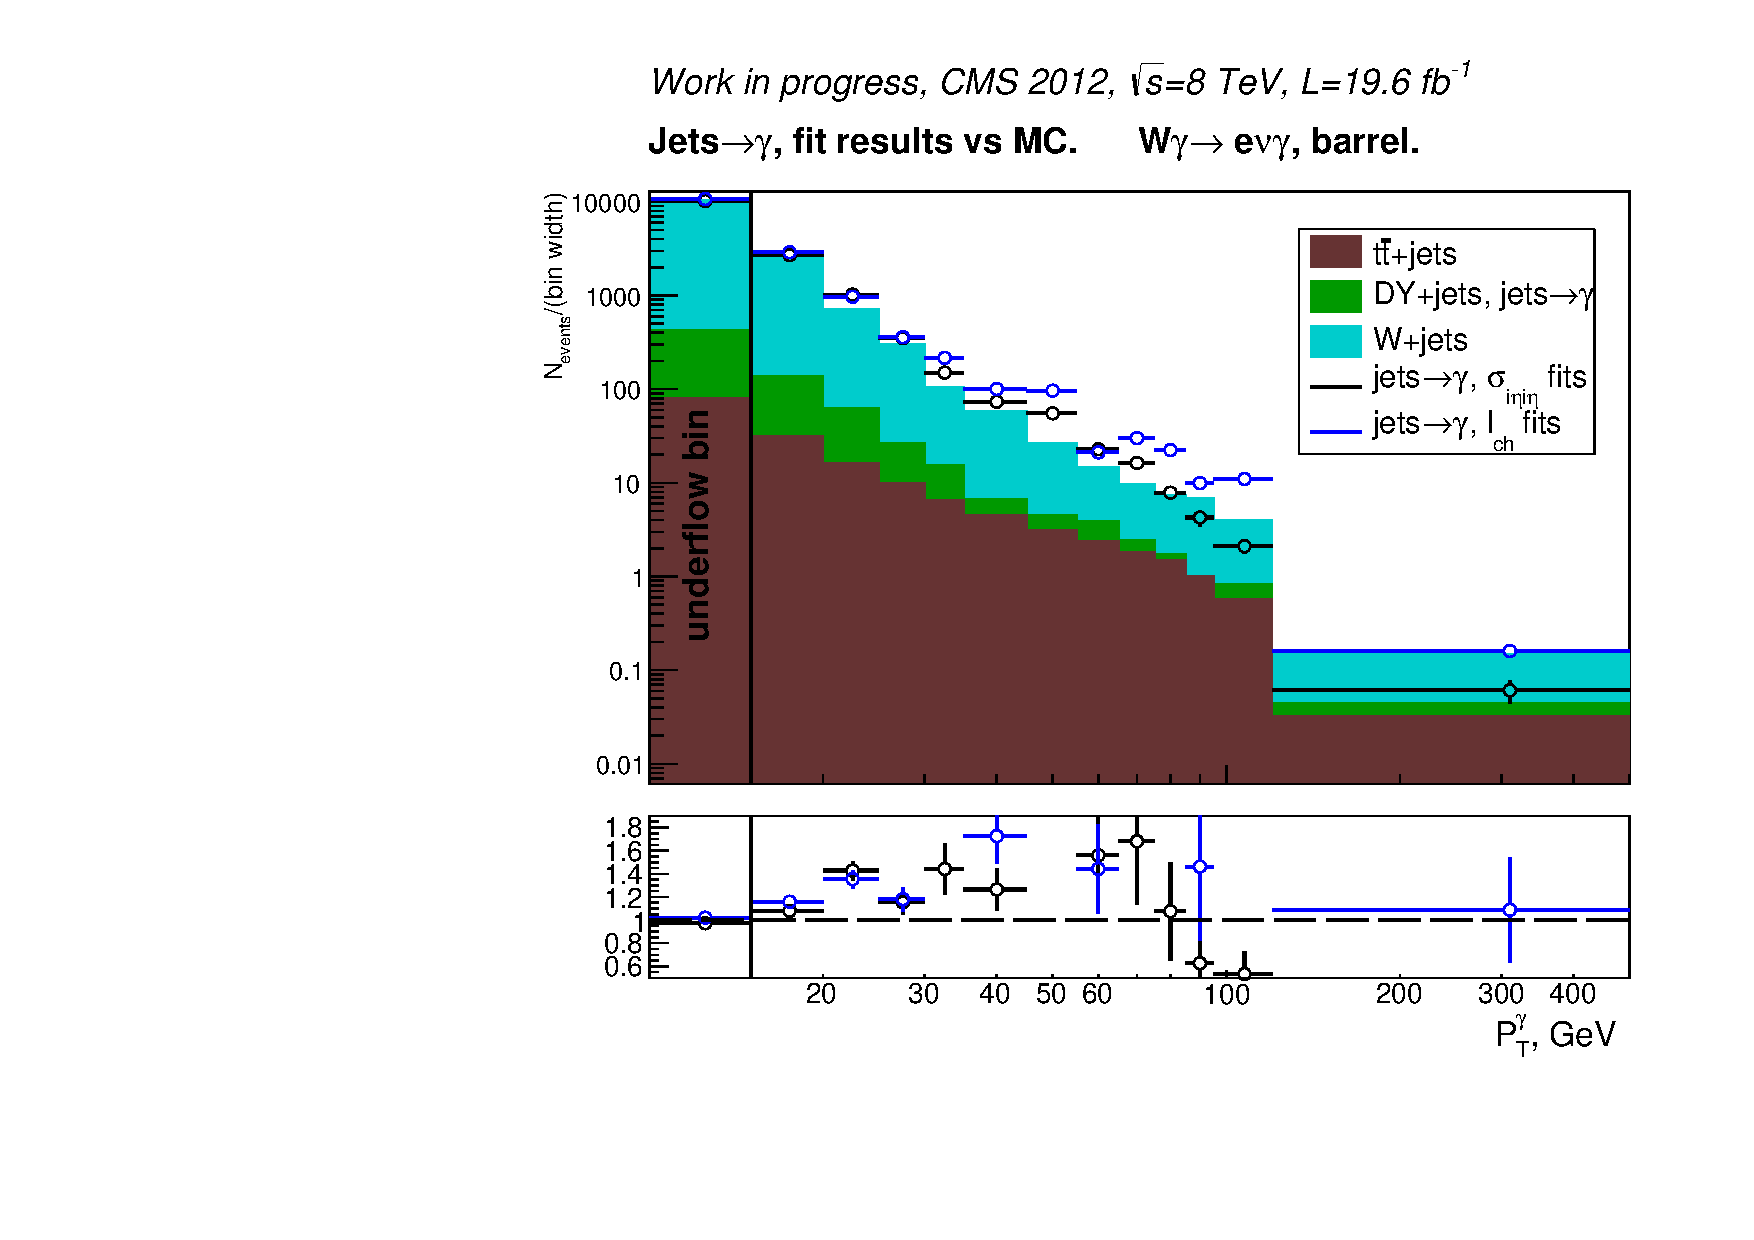
\includegraphics[width=0.45\textwidth]{../figs/figs_v11/ELECTRON_WGamma/PrepareYields/c_FakeDDvsMC_c_ELECTRON_WGamma__UNblind__Barrel__phoEt.pdf}\\
    \end{center}
  \end{figure}
\end{frame}%{$jets \rightarrow \gamma$ Background Subtraction. Plots, W$\gamma$}

\begin{frame}\frametitle{\footnotesize{$P_T^{\gamma}$ Spectrum before and after Background Subtraction. Electron Channel, Endcap}}
  \tiny{Top: data vs fake-$\gamma$ background derived from the template method + real-$\gamma$ background predicted by dedicated MC samples + signal MC, with $I_{ch}$ and $\sigma_{i\eta{i}\eta}$ used as fit variables. Bottom: left: data yields after full background subtraction vs signal MC. $I_{ch}$ vs $\sigma_{i\eta{i}\eta}$ fit results. Right: fake-$\gamma$ data driven background prediction vs MC. Plotted with the stat error only.}
  \begin{figure}[htb]
    \begin{center}
       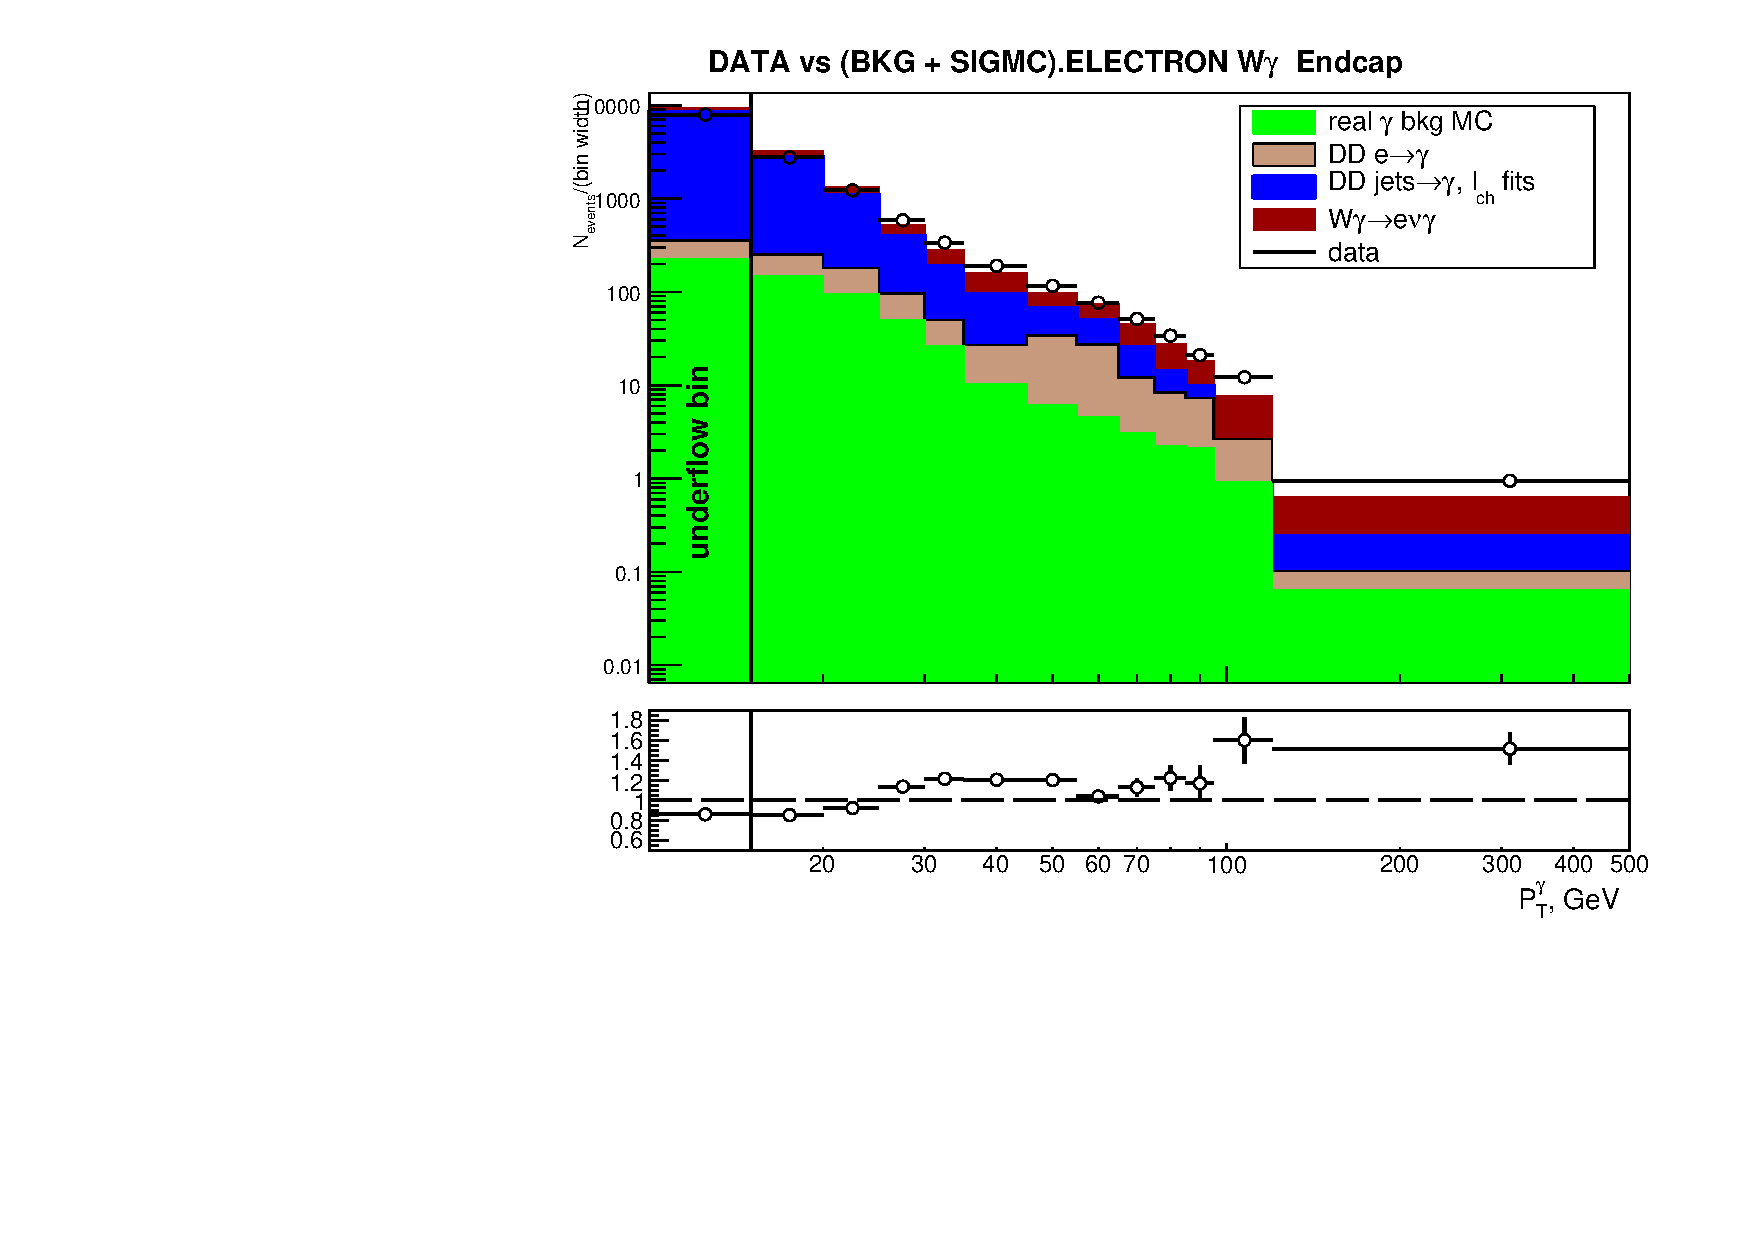
\includegraphics[width=0.45\textwidth]{../figs/figs_v11/ELECTRON_WGamma/PrepareYields/c_DATAvsBkgPlusSigMCc_ELECTRON_WGamma_TEMPL_CHISO_UNblind__Endcap__phoEt.pdf}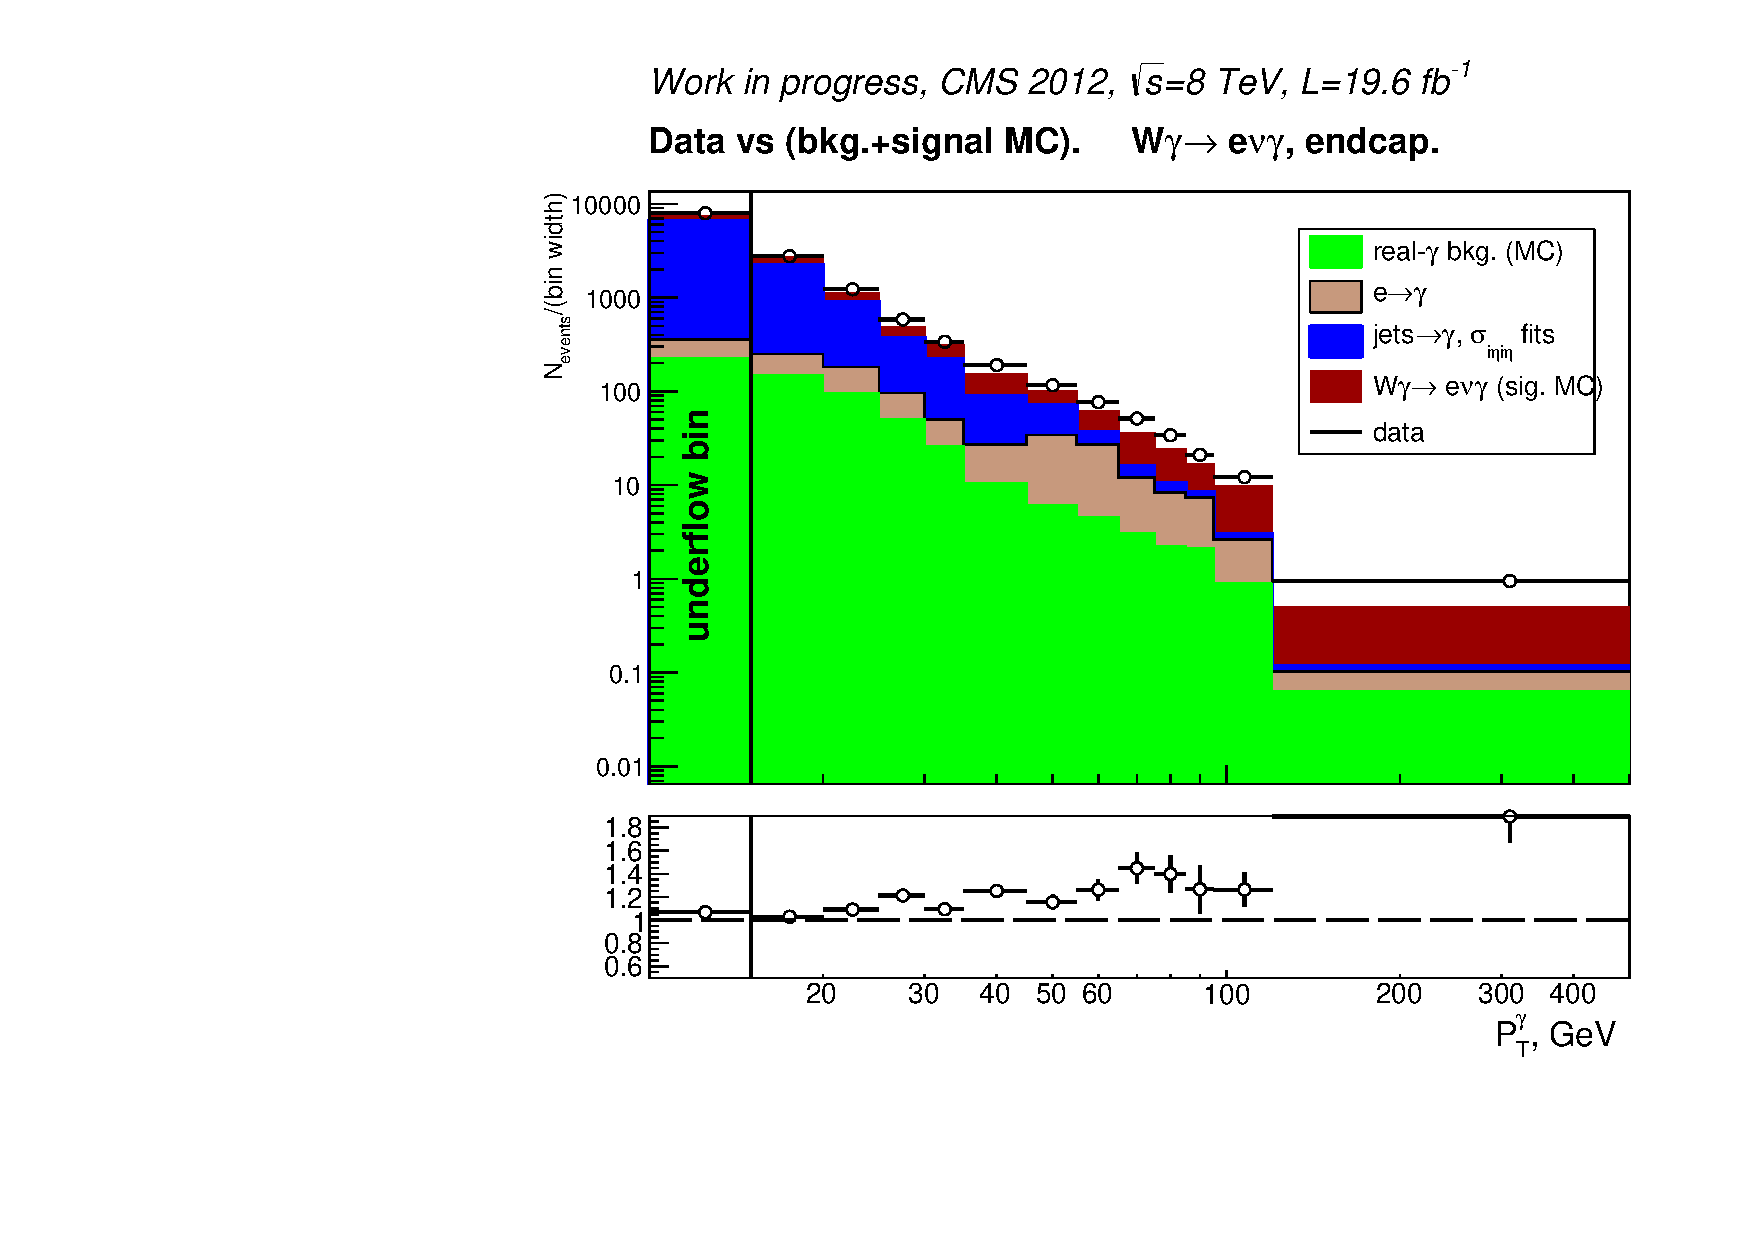
\includegraphics[width=0.45\textwidth]{../figs/figs_v11/ELECTRON_WGamma/PrepareYields/c_DATAvsBkgPlusSigMCc_ELECTRON_WGamma_TEMPL_SIHIH_UNblind__Endcap__phoEt.pdf}\\
       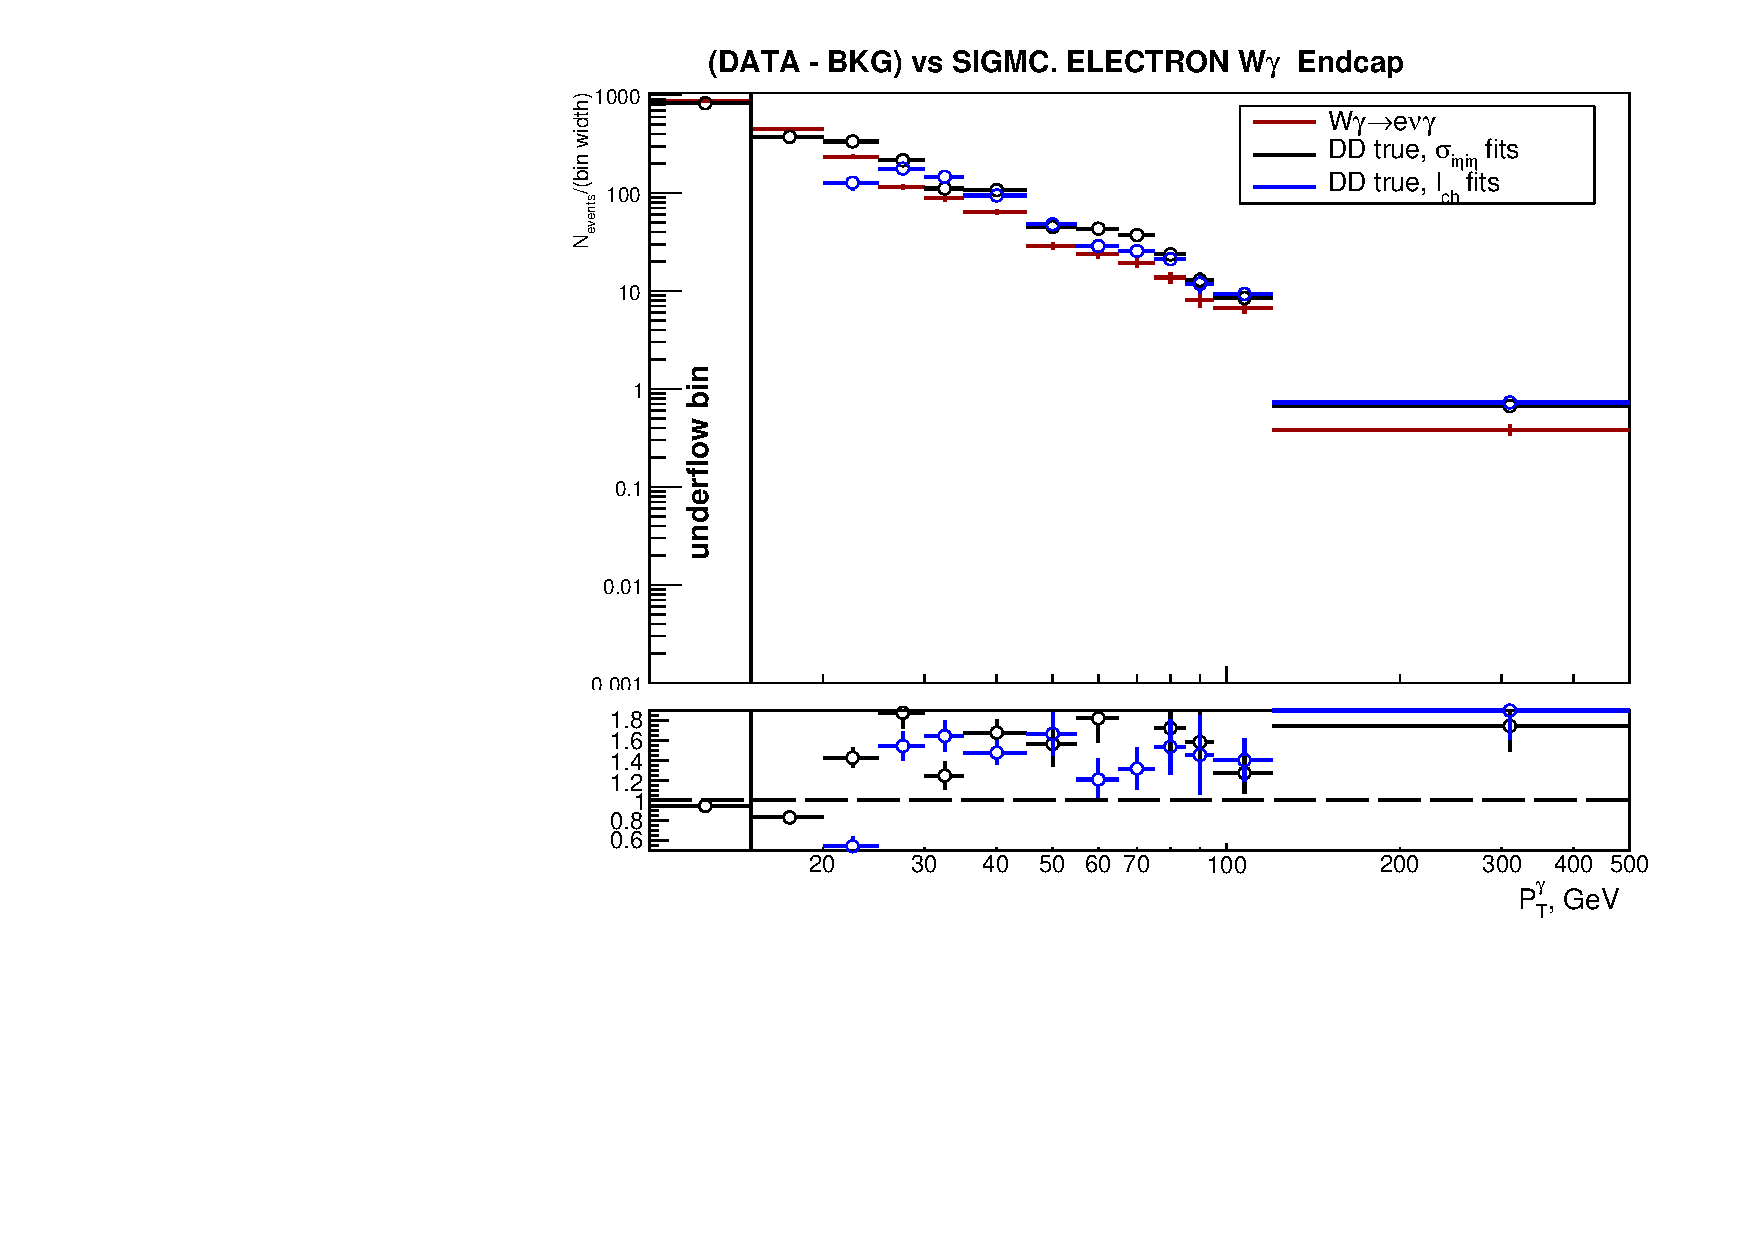
\includegraphics[width=0.45\textwidth]{../figs/figs_v11/ELECTRON_WGamma/PrepareYields/c_BkgSubtrDATAvsSIGMC_c_ELECTRON_WGamma__UNblind__Endcap__phoEt.pdf}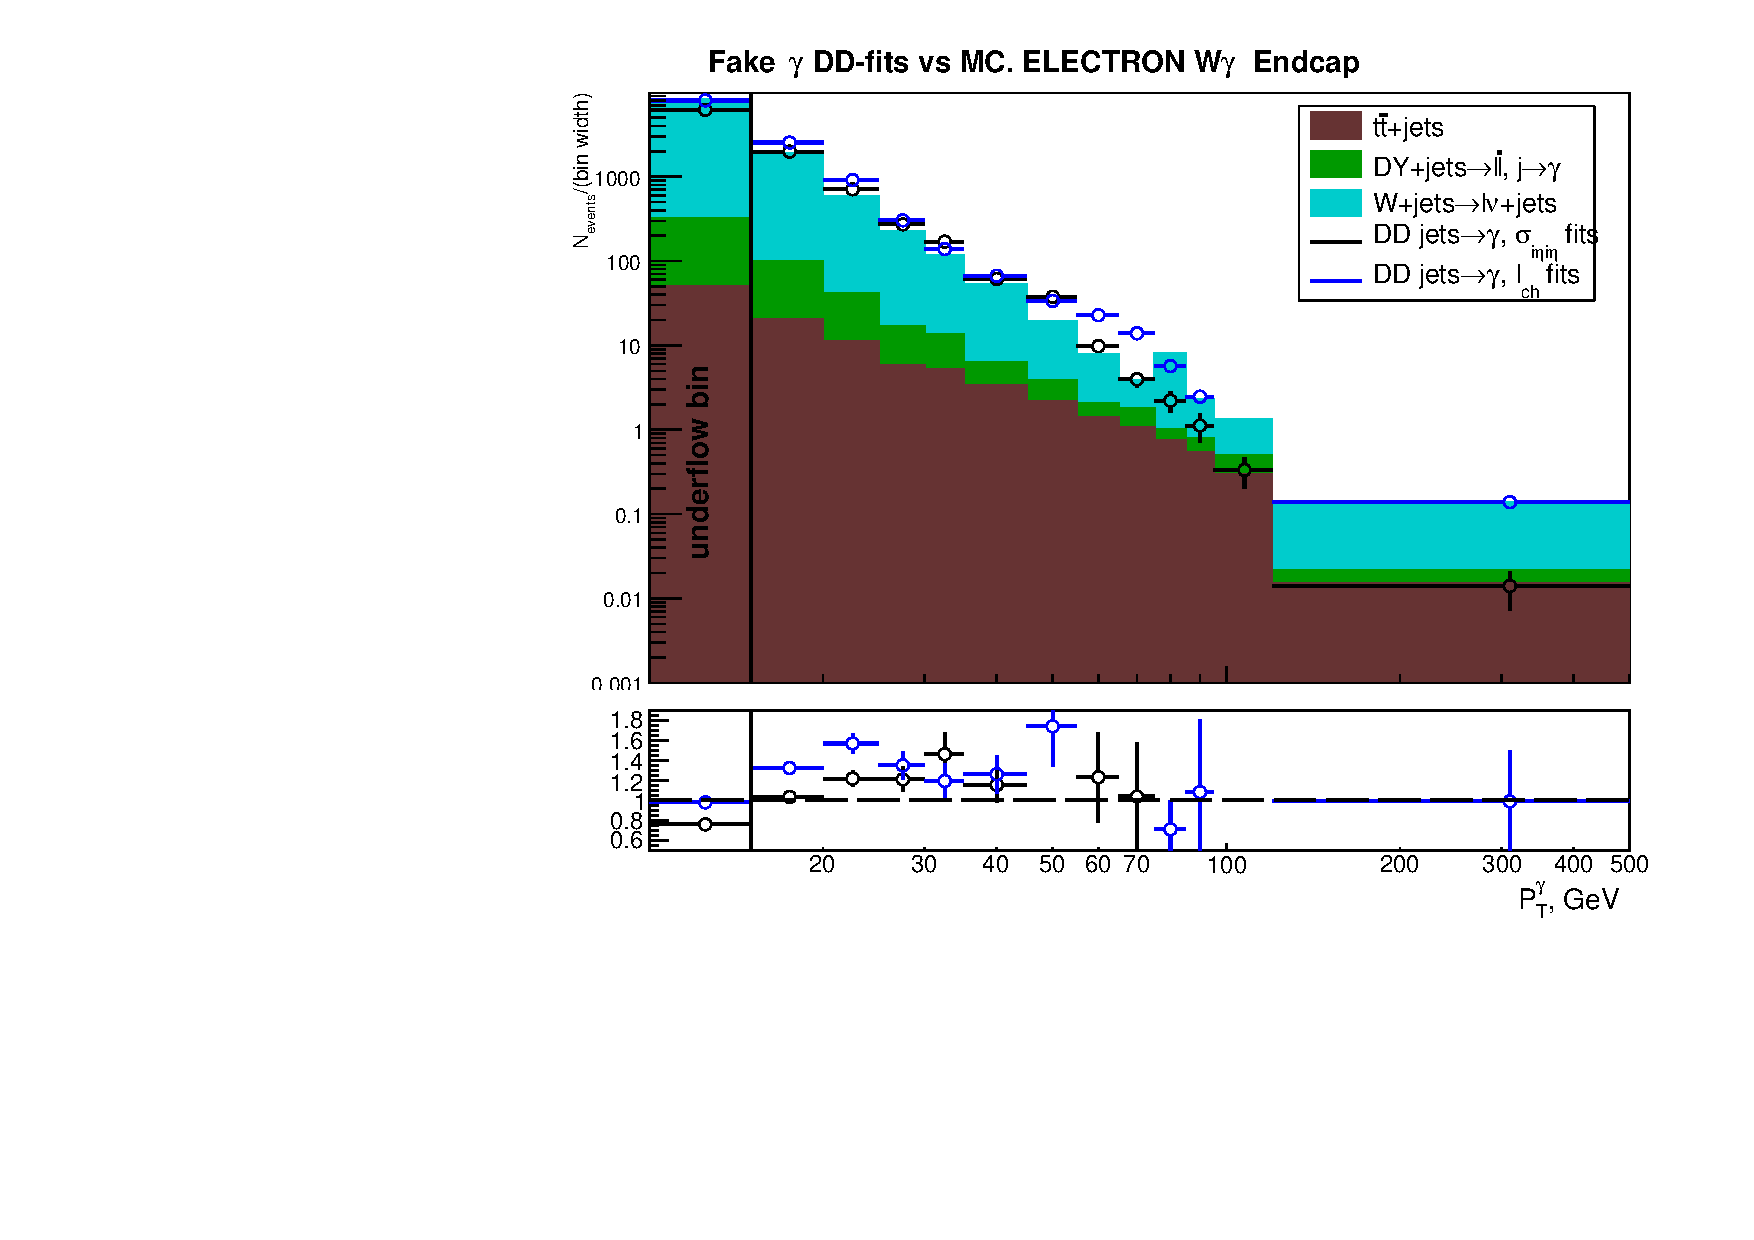
\includegraphics[width=0.45\textwidth]{../figs/figs_v11/ELECTRON_WGamma/PrepareYields/c_FakeDDvsMC_c_ELECTRON_WGamma__UNblind__Endcap__phoEt.pdf}\\
    \end{center}
  \end{figure}
\end{frame}%{$jets \rightarrow \gamma$ Background Subtraction. Plots, W$\gamma$}
